\chapter{Proofs and complements of Chapter~\ref{chap:Gand17}}
\minitoc\mtcskip


\section{Completion of the proof of Proposition \ref{prop:closureUnderPrefixSuffix}}\label{sec:prop:closureUnderPrefixSuffix}
\paragraph*{Language $\hsE_{\Ku}(\Lang(\Au))$.} Let us consider the $\NFA$ $\Au_{\hsE}$ over $S$ given by
\[\Au_{\hsE}=\tpl{S,(M\cup \{q'_0\})\times S ,\{q'_0\}\times S,\Delta',F},\]
where $q'_0\notin M$ is a fresh main state, and for all
$(q,s)\in (M\cup \{q'_0\})\times S$ and $s'\in S$, we have $\Delta'((q,s),s')=\emptyset$, if $s'\neq s$, and 
%$\Delta((q,s),s)$ is defined as follows:
%
\[
%\begin{array}{l}
\Delta((q,s),s)=  \left\{
    \begin{array}{ll}
    \Delta((q,s),s)
      &    \text{ if }  q\neq q'_0
      \\
(\{q'_0\}\times \Edges(s))\cup \{(q_0,s')\in Q_0\mid s'\in \Edges(s)\}
 &    \text{ otherwise.}
    \end{array}
  \right.
%\end{array}
\]
%
%Essentially, 
Starting from an initial state $(q'_0,s)$, the automaton $\Au_{\hsE}$ either remains in a state whose   main component is $q'_0$, or moves to an initial state $(q_0,s')$ of $\Au$, ensuring at the same time that the portion of the input read so far is faithful to the evolution of  $\Ku$. From the state $(q_0,s')$,
 $\Au_{\hsE}$ simulates the behavior of $\Au$.  Formally, since $\Au$ is a $\Ku$-\NFA,  by construction it easily follows that $\Au_{\hsE}$ is a
   $\Ku$-\NFA\ which accepts the set of traces of $\Ku$ having a non-empty proper suffix in $\Lang(\Au)$. Hence,
   $\Lang(\Au_{\hsE})=\hsE_{\Ku}(\Lang(\Au))$.
   
\paragraph*{Language  $\hsEt_{\Ku}(\Lang(\Au))$.} Let us consider the $\NFA$ $\Au_{\hsEt}$ over $S$ given by
\[\Au_{\hsEt}=\tpl{S,(M\cup \{q_\acc\})\times S ,Q'_0,\Delta',\{q_\acc\}\times S},\] where $q_\acc\notin M$ is a fresh main state, and $Q'_0$ and $\Delta'$ are defined as follows:
\begin{itemize}
  \item the set $Q'_0$ of initial states is the set of states $(q,s)$ of $\Au$ such that there is a run of $\Au$ from some initial state to $(q,s)$ over some non-empty word.
  \item For all
$(q,s)\in (M\cup \{q_\acc\})\times S$ and $s'\in S$, we have $\Delta'((q,s),s')=\emptyset$, if $s'\neq s$, and 
%
\[%\hspace{-0.3cm}
%\begin{array}{l}
\Delta'((q,s),s)=  \left\{
    \begin{array}{ll}
\Delta((q,s),s)\cup \quad  \displaystyle{\smashoperator{\bigcup_{(q',s')\in F\cap \Delta((q,s),s)}}}\; \{(q_\acc,s')\}
      &    \text{ if } q\in M
      \\
    \emptyset
      &    \text{ if } q= q_\acc.
    \end{array}
  \right.
%\end{array}
\]
%
\end{itemize}
%
Note that the set $Q'_0$ can be computed in time polynomial in the size of $\Au$. Since   $\Au_{\hsEt}$ essentially simulates $\Au$, and $\Au$ is
 a $\Ku$-\NFA, by construction we easily obtain that  $\Au_{\hsEt}$ is  a $\Ku$-$\NFA$ which accepts the set of words over $S$ which are
non-empty proper suffixes of words in $\Lang(\Au)$.
Thus, since $\Au$ is a $\Ku$-\NFA, we obtain that $\Lang(\Au_{\hsEt})=\hsEt_{\Ku}(\Lang(\Au))$.\qed
 

\section{Proof of Proposition~\ref{prop:invarianceLeftRightPrefix}}
\label{proof:prop:invarianceLeftRightPrefix}

\begin{proposition*}[\ref{prop:invarianceLeftRightPrefix}] Let $h\geq 0$, and $\rho$ and $\rho'$ be two $h$-prefix  bisimilar traces of  $\Ku$. Then, for all traces $\rho_L$ and $\rho_R$ of $\Ku$ such that $\rho_L \star \rho$ and  $\rho \star \rho_R$ are defined, the following properties hold:
\begin{enumerate}
    \item $\rho_L\star \rho$ and $\rho_L\star \rho'$ are $h$-prefix   bisimilar; 
    \item $\rho\star \rho_R$ and $\rho'\star \rho_R$ are $h$-prefix  bisimilar.
\end{enumerate}
\end{proposition*}

\begin{proof}
Let us note first that, since $\Summary(\rho)=\Summary(\rho')$, we have $\fst(\rho)=\fst(\rho')$ and $\lst(\rho)=\lst(\rho')$.
Hence $\rho_L\star \rho$ (resp., $\rho\star \rho_R$) is defined if and only if  $\rho_L\star \rho'$ (resp., $\rho'\star \rho_R$) is defined.
The proofs of $(1.)$ and $(2.)$ are by induction on $h\geq 0$.

$(1.)$ Since $\rho$ and $\rho'$ are $h$-prefix bisimilar, $\Summary(\rho)=\Summary(\rho')$. By Proposition~\ref{prop:Summaries},
 $\Summary(\rho_L\star \rho)=\Summary(\rho_L\star \rho')$. Thus, if $h=0$ (base case), the thesis follows. Now let $h>0$ (inductive step). Let us assume that $\nu$ is a proper prefix of
 $\rho_L\star\rho$ (the symmetric case, where we consider a proper prefix of $\rho_L\star \rho'$ is similar). We need to show that there exists a proper prefix $\nu'$ of
 $\rho_L\star\rho'$ such that $\nu$ and $\nu'$ are $(h-1)$-prefix bisimilar. If $\nu$ is a prefix of $\rho_L$, then we set $\nu'=\nu$ and the result trivially follows (note that, since $\rho$ and $\rho'$ are $h$-prefix bisimilar, it holds that $|\rho|>1$ if and only if $|\rho'|>1$). Otherwise, there is a proper prefix $\xi$ of $\rho$ such that
 $\nu=\rho_L\star \xi$. Since $\rho$ and $\rho'$ are $h$-prefix bisimilar, there exists a proper prefix $\xi'$ of $\rho'$ such that $\xi$ and $\xi'$ are $(h-1)$-prefix bisimilar.
Thus, by setting $\nu'=\rho_L\star \xi'$, by the inductive hypothesis the thesis follows.

$(2.)$ By Proposition~\ref{prop:Summaries},
 $\Summary(\rho\star \rho_R)=\Summary(\rho'\star \rho_R)$. Thus, if $h=0$, the thesis follows. Now, let us assume that $h>0$.
We proceed by a double  induction on $|\rho_R|$. As for the base case, where $|\rho_R|=1$, the result is obvious. Thus let us assume that $|\rho_R|>1$.
  Let $\nu$ be a proper prefix of
 $\rho\star\rho_R$ (the symmetric case, where we consider a proper prefix of $\rho'\star \rho_R$ is similar). We need to show that there exists a proper prefix $\nu'$ of
 $\rho'\star\rho_R$ such that $\nu$ and $\nu'$ are $(h-1)$-prefix bisimilar. If $\nu=\rho$ or $\nu$ is a proper prefix of $ \rho$, then there exists a prefix $\nu'$ of
 $ \rho'$ such that $\nu$ and $\nu'$ are $(h-1)$-prefix bisimilar. Thus, since $\nu'$ is a proper prefix of $\rho'\star\rho_R$, the result follows.
 Otherwise, there exists a proper prefix $\xi$ of $\rho_R$ such that
 $\nu=\rho\star \xi$. By setting $\nu'=\rho'\star\xi$, and considering the inductive hypothesis on $|\rho_R|$, we obtain that $\nu$ and $\nu'$ are $h$-prefix bisimilar,
 hence $(h-1)$-prefix bisimilar as well, concluding the proof.
\end{proof}


\section{Proof of Proposition~\ref{prop:fulfillmentPreservingPrefix}}
\label{proof:prop:fulfillmentPreservingPrefix}

\begin{proposition*}[\ref{prop:fulfillmentPreservingPrefix}] Let $h\geq 0$, and $\rho$ and $\rho'$ be two $h$-prefix bisimilar traces of $\Ku$. Then, for each $\AAbarBBbarEbar$
formula $\psi$ over $\SPEC$ with $\nestb(\psi)\leq h$, we have that
\[\Ku,\rho\models\psi\iff \Ku,\rho'\models\psi.\]
\end{proposition*}

\begin{proof}
We prove the proposition by a nested induction on the structure of the formula $\psi$ and on the B-nesting depth $\nestb(\psi)$. 

As for the base case, $\psi$ is a regular expression in $\SPEC$. Since $\Summary(\rho)=\Summary(\rho')$ (as $\rho$ and $\rho'$ are $h$-prefix bisimilar) the thesis holds  by Proposition~\ref{prop:Summaries}.

Let us now consider the inductive step.
%$|\psi|>1$. 
The cases where the root modality of $\psi$ is a Boolean connective directly follow by the inductive hypothesis.
As for the cases where the root modality is $\hsA$ or $\hsAt$, the result follows from the fact that, being $\rho$ and $\rho'$ $h$-prefix bisimilar, we have
$\fst(\rho)=\fst(\rho')$ and $\lst(\rho)=\lst(\rho')$.
It remains to consider the cases where the root modality is  $\hsB$, $\hsBt$, or $\hsEt$. We prove the implication
$\Ku,\rho\models \psi \Longrightarrow \Ku,\rho'\models \psi$ (the converse is similar).  Let
$\Ku,\rho\models \psi$. %We need to show that $\Ku,\rho'\models \psi$.
\begin{itemize}
  \item $\psi=\hsB\varphi$: since $0<\nestb(\psi)\leq h$,  it holds that $h>0$.  As $\Ku,\rho\models\hsB\varphi$,   there is a proper prefix $\nu$ of $\rho$  such that $\Ku,\nu\models\varphi$.
  Since $\rho$ and $\rho'$ are $h$-prefix bisimilar, there is a proper prefix $\nu'$ of $\rho'$ such that $\nu$ and $\nu'$ are $(h-1)$-prefix bisimilar.
  Being $\nestb(\varphi)\leq h-1$, by the inductive hypothesis we obtain that  $\Ku,\nu'\models\varphi$. Hence,  $\Ku,\rho'\models\hsB\varphi$.
  \item $\psi=\hsBt\varphi$: since $\Ku,\rho\models\hsBt\varphi$, there is a trace $\rho_R$ such that $|\rho_R|>1$ and
$\Ku,\rho\star\rho_R\models\varphi$. By Proposition~\ref{prop:invarianceLeftRightPrefix}, $\rho\star\rho_R$ and $\rho'\star\rho_R$ are $h$-prefix bisimilar. By the inductive hypothesis on  the structure of the formula, we obtain that $\Ku,\rho'\star\rho_R\models\varphi$. Hence,
  $\Ku,\rho'\models\hsBt\varphi$. %, and the result follows.
  \item    $\psi=\hsEt\varphi$: this case is similar to the previous one.\qedhere % since $\Ku,\rho\models\hsEt\varphi$, there exists a trace $\rho''$ such that $|\rho''|>1$ and
%$\Ku,\rho''\star\rho\models\varphi$. By Proposition~\ref{prop:invarianceLeftRightPrefix}, $\rho''\star\rho$ and $\rho''\star\rho'$ are $h$-prefix bisimilar. Thus, by the induction hypothesis on  the structure of the formula, $\Ku,\rho''\star\rho'\models\varphi$. Hence,
%  $\Ku,\rho'\models\hsEt\varphi$, and the result follows.
\end{itemize}
\end{proof}


\section{Proof of Lemma~\ref{lemma:prefixSamplingOneRegex}}\label{proof:lemma:prefixSamplingOneRegex}

\begin{lemma*}[\ref{lemma:prefixSamplingOneRegex}] For $h\geq 0$, any two traces
$\rho$ and  $\rho'$ of $\Ku$ having the same
$h$-sampling word are $h$-prefix bisimilar.
\end{lemma*}

\begin{proof}
The proof can be immediately derived by a stronger result stated in the following claim.
%
\begin{claim}\label{lab:clAux} Let $h\geq 0$,  $\rho$ and  $\rho'$ be two traces of $\Ku$, and $\PrefS_h$ and $\PrefS'_h$ be the two $h$-prefix samplings
of $\rho$ and $\rho'$, resp.. Assume that $\rho$ and $\rho'$ have the same $h$-sampling word, namely there is $N\geq 1$ such that
 \begin{itemize}
   \item 
   $\PrefS_h: i_1<i_2<\ldots < i_N$,
   \item 
   $\PrefS'_h: i'_1<i'_2<\ldots < i'_N$, and
   \item 
  for all $j\in [1,N]$, $\Summary(\rho(1,i_j))=\Summary(\rho'(1,i'_j))$.
 \end{itemize}

 Then, for all $j\in [1,N-1]$, $n\in [i_j+1,i_{j+1}]$ and $n'\in [i'_j+1,i'_{j+1}]$ such that $\Summary(\rho[1,n])=\Summary(\rho'[1,n'])$, it holds that
 $\rho(1,n)$ and $\rho'(1,n')$ are $h$-prefix bisimilar.
\end{claim}
\begin{proof} The proof is by induction on $h\geq 0$. For $h=0$, the result is obvious. Now let us assume that $h>0$. If $N=1$ (resp., $N=2$), then
$\rho=\rho'$  and $|\rho|=|\rho'|=N$, and the thesis trivially holds.
Now, let us assume that $N>2$. Since by hypothesis $\Summary(\rho(1,n))=\Summary(\rho'(1,n'))$, we need to show that:
 \begin{enumerate}
   \item for each $m\in [1,n-1]$, there exists $m'\in [1,n'-1]$ such that $\rho(1,m)$ and $\rho'(1,m')$ are $(h-1)$-prefix bisimilar;
   \item for each $m'\in [1,n'-1]$, there exists $m\in [1,n-1]$ such that $\rho(1,m)$ and $\rho'(1,m')$ are $(h-1)$-prefix bisimilar;
 \end{enumerate}
We only prove $(1.)$, being the proof of $(2.)$ symmetric. We exploit in the proof the following fact that can be easily shown:
%
let $k\in [0,h-1]$ and $1=x_1<\ldots <x_r=N$ be the subsequence of $1,\ldots,N$ such that
$i_{x_1}<\ldots<i_{x_r}$ is the $k$-prefix sampling of $\rho$. Then, $i'_{x_1}<\ldots<i'_{x_r}$ is the $k$-prefix sampling of $\rho'$.

Now we prove $(1.)$. Let $m\in [1,n-1]$. If $m=1$, we set $m'=1$, and the result follows.
Now, let us assume that $m\geq 2$. Since $h>0$, there must exist $x,y\in [1,N]$ such that $x<y$, $m\in [i_{x}+1,i_y]$, and $i_x$ and $i_y$ are two consecutive positions in the
$(h-1)$-prefix sampling of $\rho$. By the fact above, $i'_x$ and $i'_y$ are two consecutive positions in the $(h-1)$-prefix sampling of $\rho'$. We distinguish two cases:
\begin{itemize}
\item $m=i_y$. Since $n\in [i_j+1,i_{j+1}]$ and $m<n$, it holds that $i_y\leq i_j$. Hence, $i'_y\leq i'_j$ as well. Moreover, since $n'>i'_j$, it holds that $i'_y<n'$.
We set $m'=i'_y$. As $\Summary(\rho(1,i_y))=\Summary(\rho'(1,i'_y))$, $m=i_y$, $m'=i'_y$, and $i_x$ and $i_y$ (resp., $i'_x$ and $i'_y$) are two consecutive positions in
the $(h-1)$-prefix sampling of $\rho$ (resp., $\rho'$), the thesis follows by the inductive hypothesis on $h$.
\item $m\neq i_y$. Hence, $m\in [i_x+1,i_y-1]$. Since $i_x$ and $i_y$ are two consecutive positions in the $(h-1)$-prefix sampling of $\rho$, there must exist $z\in [x+1,y-1]$
such that $i_z\leq m$ and $\Summary(\rho(1,m))=\Summary(\rho(1,i_z))$. Since $i_z\leq m$, $m<n$, and $n\in [i_j+1,i_{j+1}]$, it holds that $i_z\leq i_j$.
Hence, $i'_z\leq i'_j<n'$. We set $m'=i'_z$. As $\Summary(\rho(1,i_z))=\Summary(\rho'(1,i'_z))$, we obtain that
$\Summary(\rho(1,m))=\Summary(\rho'(1,m'))$, $m\in [i_{x}+1,i_y]$ and $m'\in [i'_x+1,i'_y]$. Thus, being  $i_x$ and $i_y$ (resp., $i'_x$ and $i'_y$)   two consecutive positions in the $(h-1)$-prefix sampling of $\rho$ (resp., $\rho'$), by the inductive hypothesis on $h$ the result follows. \qedhere
\end{itemize}
\end{proof}
This concludes the proof of the claim, and of  Lemma~\ref{lemma:prefixSamplingOneRegex} as well.
\end{proof}


\section{Pseudocode of \texttt{checkFalse}}\label{sec:chkFalse}
The pseudocode of procedure $\texttt{checkFalse}$, the \lq\lq dual\rq\rq{} of $\texttt{checkTrue}$, 
is reported in Algorithm~\ref{fig-proc-checkFALSE} at page~\pageref{fig-proc-checkFALSE}.

\begin{algorithm}[p]
\caption{$\texttt{checkFalse}_{\tpl{\Ku,\varphi,\GLab}}(\WS)$}\label{fig-proc-checkFALSE}
%\begin{multicols}{2}
\begin{algorithmic}[1]
\While{$\WS$ is \emph{not} universal}
    \State{deterministically select $(\psi,\rho)\in \WS$ s.t. $\psi$ is not of the form  $\hsEtu\psi'$ and $\hsBtu\psi'$}
    \State{$\WS\leftarrow \WS\setminus \{(\psi,\rho)\}$}
    \Case{ $\psi=r$  with $r\in \RE$}
        \If{$\rho\notin \Lang(r)$}
            \State{accept the input}
        \EndIf
    \case{ $\psi=\neg r$ with $r\in \RE$}
        \If{$\rho\in \Lang(r)$}
            \State{accept the input}
        \EndIf
    \case{ $\psi=\hsA \psi'$ or $\psi=\hsAu \psi'$}
        \If{$\psi\notin\GLab(\lst(\rho))$}
            \State{accept the input}
        \EndIf
    \case{ $\psi=\hsAt \psi'$ or $\psi=\hsAtu \psi'$}      \If{$\psi\notin\GLab(\fst(\rho))$}
            \State{accept the input}
        \EndIf
    \case{ $\psi=\psi_1\vee \psi_2$}
        \State{universally choose $i=1,2$}
        \State{$\WS\leftarrow \WS\cup \{(\psi_i,\rho)\}$}
        
%\columnbreak        
        
    \case{ $\psi=\psi_1\wedge \psi_2$}
        \State{$\WS\leftarrow \WS\cup \{(\psi_1,\rho),(\psi_2,\rho)\}$}
    \case{ $\psi=\hsB\psi'$}
        \State{universally choose $\rho'\in \Pref(\rho)$}
        \State{$\WS\leftarrow \WS\cup \{(\psi',\rho')\}$}
    \case{ $\psi=\hsBu\psi'$}
        \State{$\WS\leftarrow \WS\cup \{(\psi',\rho')\mid \rho'\in\Pref(\rho)\}$}
    \case{ $\psi=\hsX\psi'$ with $X\in \{\overline{E},\overline{B}\}$}
        \State{universally choose an $X$-\emph{witness} $\rho'$ of $\rho$ for $(\Ku,\varphi)$}
        \State{$\mathcal{\WS}\leftarrow \mathcal{\WS}\cup \{(\psi',\rho')\}$}
    \EndCase
\EndWhile
% 
\If{$\mathcal{\WS}=\emptyset$}
    \State{reject the input}
\Else
    \State{existentially choose $(\psi,\rho)\in \widetilde{\WS}$}
    \State{$\texttt{checkTrue}_{\tpl{\Ku,\varphi,\GLab}}(\{(\psi,\rho)\})$}
\EndIf
\end{algorithmic}
%\end{multicols}
\end{algorithm}

 
\section{Proof of Proposition~\ref{prop:correctnessATMcheck}}\label{APP:correctnessATMcheck}

For technical convenience, given an $\AAbarBBbarEbar$ formula $\varphi$, we consider a slight variant $\Alt(\varphi)$ of $\AltN(\varphi)$. Formally, $\Alt(\varphi)$ is defined as $\AltN(\hsBt\varphi)$ (or, equivalently, as $\AltN(\hsEt\varphi)$).
Note that for each
$\AAbarBBbarEbar$ formula $\varphi$ and $X\in \{\overline{E},\overline{B}\}$, we have $\Alt(\hsXu\varphi)=\Alt(\widetilde{\hsXu\varphi})+1$.

Let $\Ku$ be a finite Kripke structure,  $\varphi$
be an $\AAbarBBbarEbar$ formula in \nnf, and $\WS$ be a well-formed set for $(\Ku,\varphi)$.
We denote by $\Alt(\WS)$ the maximum over the  alternation depths $\Alt(\psi)$, where $\psi$ is a formula occurring in $\WS$
(we set $\Alt(\WS)=0$ if $\WS=\emptyset$).
For each non-empty \emph{universal} well-formed set $\WS$ for $(\Ku,\varphi)$, we have $\Alt(\widetilde{\WS})= \Alt(\WS)- 1$.

Now, we can prove Proposition~\ref{prop:correctnessATMcheck}.
\begin{proposition*}[\ref{prop:correctnessATMcheck}] The ATM  $\texttt{check}$ is a singly exponential-time bounded ATM accepting $\FMC$ whose number of alternations on input $(\Ku,\varphi)$ is at most $\AltN(\varphi)+2$.
\end{proposition*}
\begin{proof}
Let us fix an input $(\Ku,\varphi)$, where $\varphi$
is an $\AAbarBBbarEbar$ formula in \nnf. 

Note that whenever there is a switch between the procedures $\texttt{checkTrue}$ and $\texttt{checkFalse}$, e.g., from $\texttt{checkTrue}$ to $\texttt{checkFalse}$, $(i)$~the input $\{(\psi,\rho)\}$ of the called procedure is contained in the dual $\widetilde{\WS}$ of the currently processed well-formed set $\WS$ for $(\Ku,\varphi)$, and $(ii)$~$\WS$ is non-empty and universal, hence $\Alt(\{(\psi,\rho)\})< \Alt(\WS)$. Moreover, a well-formed set $\WS$ for $(\Ku,\varphi)$ contains only formulas $\psi$ such that $\psi\in \SD(\varphi)$.

Additionally, in each iteration of the while loops of procedures $\texttt{checkTrue}$ and $\texttt{checkFalse}$, the processed pair $(\psi,\rho)$ in the current well-formed set $\WS$ is either removed from $\WS$, or it is replaced with pairs $(\psi',\rho')$ such that $\psi'$ is a strict subformula of $\psi$.
 This ensures that the algorithm always terminates. 
 
Furthermore, since the number of alternations of the ATM $\texttt{check}$  between existential choices and universal choices is evidently the number of switches between the calls to procedures $\texttt{checkTrue}$ and $\texttt{checkFalse}$ plus 2, and the top calls to $\texttt{checkTrue}$ take as input well-formed sets for $(\Ku,\varphi)$ having the form  $\{(\psi,\rho)\}$, where $\psi\in\SD(\varphi)$, we have proved the following result.

\begin{claim}
The number of alternations of the ATM \texttt{check} on input $(\Ku,\varphi)$ is at most $\AltN(\varphi)+2$.
\end{claim} 

Next, we prove the following property.
\begin{claim}\label{claim:sinExp}
The ATM $\texttt{check}$ runs in time singly exponential in the size of the input $(\Ku,\varphi)$.
\end{claim}
\begin{proof}
Let us fix an input $(\Ku,\varphi)$.  Let $T(\varphi)$ be the standard tree encoding of $\varphi$, where each node is labeled by some subformula of $\varphi$.
Let $\psi\in\SD(\varphi)$. If $\psi$ is a subformula of $\varphi$, we define $d_\psi$ as the maximum over the distances from the root in $T(\varphi)$ of $\psi$-labeled nodes. If, conversely, $\psi$ is the dual of a subformula of $\varphi$, we let
 $d_\psi = d_{\widetilde{\psi}}$. 
 
Let us denote by $H(\Ku,\varphi)$ the length of a certificate for $(\Ku,\varphi)$. Recall that   $H(\Ku,\varphi)= (|\States|\cdot 2^{(2|\SPEC|)^2})^{h+2}$,
  where $\States$ is the set of states of $\Ku$,  $\SPEC$ is the set of atomic formulas (regular expressions) occurring in $\varphi$, and $h=\nestb(\varphi)$.

By Proposition~\ref{prop:EbarBbarWitness},  it follows that each  step in an iteration of the while loops in the procedures $\texttt{checkTrue}$ and $\texttt{checkFalse}$ can be performed in time singly exponential in the size of $(\Ku,\varphi)$.
 Thus, in order to prove Claim~\ref{claim:sinExp},  it suffices to show that
for all  computations $\pi$ of the ATM $\texttt{check}$ starting from the input $(\Ku,\varphi)$, the overall number $N_\psi$ of iterations of the while loops (of procedures $\texttt{checkTrue}$ and $\texttt{checkFalse}$) along $\pi$, where the formula $\psi$ is processed, is at most $(2^{|\varphi|}\cdot H(\Ku,\varphi))^{d_\psi}$. 

The proof is done by induction on $d_\psi$. As for the base case, we have $d_\psi = 0$. Therefore, $\psi=\varphi$ or $\psi=\widetilde{\varphi}$; by construction of the algorithm, $N_\varphi$ and $N_{\widetilde{\varphi}}$ are at most equal to $1$. Thus the result holds. 

As for the inductive step, let us assume that  $d_\psi > 0$. We consider the case where $\psi$ is a subformula of $\varphi$ (the case where $\widetilde{\psi}$ is a subformula of $\varphi$ is similar). Then, the result follows from the next sequence of inequalities, where $P(\psi)$ denotes the set of  nodes of $T(\varphi)$ which are parents of the nodes labeled by $\psi$, and for each node $x$, $\textit{fo}(x)$ denotes the formula labeling $x$.
\begin{multline*}
N_\psi  \leq  \sum_{x\in P(\psi)} N_{\textit{fo}(x)} \cdot H(\Ku,\varphi) \leq \\
\leq \sum_{x\in P(\psi)} (2^{|\varphi|}\cdot H(\Ku,\varphi))^{d_{\textit{fo}(x)}} \cdot H(\Ku,\varphi) \leq \big(2^{|\varphi|}\cdot H(\Ku,\varphi)\big)^{d_\psi}.
\end{multline*}
%
The first inequality directly follows from the construction of the algorithm (note that if $\textit{fo}(x)=\hsBu\psi$, the processing of the subformula $\textit{fo}(x)$ in an iteration of the two while loops generates at most  $H(\Ku,\varphi)$ new ``copies'' of $\psi$). The second inequality follows by the inductive hypothesis, and the last one from the fact that $|P(\psi)|\leq 2^{|\varphi|}$  and $d_{\textit{fo}(x)}\leq d_{\psi} -1$ for all $x\in P(\psi)$. This concludes the proof of Claim~\ref{claim:sinExp}. 
\end{proof}

It remains to show that the ATM $\texttt{check}$ accepts $\FMC$.  Let us fix an input $(\Ku,\varphi)$ and let $\GLab$ be the  $\AAbar$-labeling initially and existentially guessed by
$\texttt{check}$ (at line 1).
 Evidently, after the top  calls  to $\texttt{checkTrue}$,  each configuration of the procedure $\texttt{check}$  can be described by a tuple $(\ell,\GLab, \WS, f)$, where: 
 \begin{itemize}
     \item $\WS$ is a well-formed set for $(\Ku,\varphi)$,
     \item $f=\true$ if $\WS$ is processed within $\texttt{checkTrue}$, and $f=\false$ otherwise, and
     \item $\ell$ is an instruction label corresponding to one of the instructions of the procedures $\texttt{checkTrue}$ and $\texttt{checkFalse}$.
 \end{itemize}
We denote by $\ell_0$ the label associated with the while instruction. A \emph{main configuration} is a configuration having label $\ell_0$. 

Let $\GLab_\WS$ be the restriction of $\GLab$
to the set of formulas in $\AAbar(\varphi)$ which are subformulas of formulas occurring in $\WS$. In other words, for each state $s$,
$\GLab_\WS(s)$ contains all and only the formulas $\psi\in \GLab(s)$ such that either $\psi$ or its dual $\widetilde{\psi}$
is a subformula of some formula occurring in $\WS$. $\GLab_\WS$ is said to be \emph{valid} if, for all states $s$ and $\psi\in \GLab_\WS(s)$, it holds $\Ku,s\models \psi$.

\newcommand{\Norm}[1]{\ensuremath{\|{#1}\|}}

\begin{claim}\label{claim:mainconf}
Let $\WS$ be a  well-formed set  for $(\Ku,\varphi)$ and let us assume that $\GLab_\WS$ is valid. Then
\begin{enumerate}
  \item the main configuration $(\ell_0,\GLab, \WS,\true)$ leads to acceptance \emph{if and only if} $\WS$ is valid;
  \item the main configuration $(\ell_0,\GLab, \WS,\false)$ leads to acceptance \emph{if and only if} $\WS$ is \emph{not} valid.
\end{enumerate}
\end{claim} 
\begin{proof}
 We associate with $\WS$  a natural number $\Norm{\WS}$ defined as follows. Let us fix an ordering $\psi_1,\ldots,\psi_k$ of the formulas in $\SD(\varphi)$  such that, for all $i\neq j$,  $|\psi_i|>|\psi_j|$ implies $i<j$. 
 
First, we associate with $\WS$ a $(k+1)$-tuple $\tpl{n_0,n_1,\ldots,n_k}$ of natural numbers defined as: the first component $n_0$ in the tuple is the alternation depth $\Alt(\WS)$ and,
  for all the other components $n_i$, with $1\leq i\leq k$, $n_i$ is the number of elements of $\WS$ associated with the formula $\psi_i$ (i.e., the number of elements having the form $(\psi_i,\rho)$).
 
 Then $\Norm{\WS}$ is the position of the tuple $\tpl{n_0,n_1,\ldots,n_k}$ along the total lexicographic ordering over $\Nat^{k+1}$. Note that if $\WS$ is non-empty and universal, since $\Alt(\widetilde{\WS})<\Alt(\WS)$, it holds that $\Norm{\widetilde{\WS}}<\Norm{\WS}$. Moreover, $\Norm{\WS}$ strictly decreases at each iteration of the while loops   in the procedures
$\texttt{checkTrue}$ and $\texttt{checkFalse}$ (this is because at each iteration $\Alt(\WS)$ does not increase, and  an element of $\WS$ is replaced with elements associated with smaller formulas).

The proof of Claim~\ref{claim:mainconf} is now carried out by induction on $\Norm{\WS}$. As for the base case we have  $\Norm{\WS}=0$, thus $\WS$ is empty and clearly valid. By construction $\texttt{checkTrue}$ accepts the empty set, while  $\texttt{checkFalse}$ rejects the empty set.
The result holds. 

As for the inductive step, let $\Norm{\WS}>0$, hence $\WS$ is not empty.
First, we assume that $\WS$ is universal. Recall that $\Norm{\widetilde{\WS}}<\Norm{\WS}$.  Thus,
\begin{itemize}
  \item
   $\WS$ is valid $\Longleftrightarrow$   for each $(\psi,\rho)\in \widetilde{\WS}$,
    $\{(\psi,\rho)\}$ is not valid  $\Longleftrightarrow$ (by the inductive hypothesis) for each $(\psi,\rho)\in \widetilde{\WS}$, the main configuration $(\ell_0,\GLab,\allowbreak\{(\psi,\rho)\},\false)$ leads to acceptance $\Longleftrightarrow$ (by construction of the algorithm and since $\WS$ is universal) the main configuration $(\ell_0,\GLab,\WS,\true)$ leads to acceptance.
  \item  
   $\WS$ is \emph{not}  valid $\Longleftrightarrow$   for some $(\psi,\rho)\in \widetilde{\WS}$,
    $\{(\psi,\rho)\}$ is  valid  $\Longleftrightarrow$ (by the inductive hypothesis) for some $(\psi,\rho)\in \widetilde{\WS}$, the main configuration $(\ell_0,\GLab,\allowbreak \{(\psi,\rho)\},\true)$ leads to acceptance $\Longleftrightarrow$ (by construction of the algorithm and since $\WS$ is universal) the main configuration $(\ell_0,\GLab,\WS,\false)$ leads to acceptance.
\end{itemize}
%
Hence, (1.) and (2.) of Claim~\ref{claim:mainconf} hold if $\WS$ is universal. 

Now, let us assume that the non-empty set  $\WS$ is not universal.
We consider (2.) of Claim~\ref{claim:mainconf} (the proof of (1.) is just the \lq\lq dual\rq\rq).
 Let $(\psi,\rho)\in \WS$ be the pair selected by the procedure $\texttt{checkFalse}$   in the iteration of the while loop   associated with the main configuration $(\ell_0,\GLab, \WS, \false)$. Here we examine the cases where either $\psi=\hsA\psi'$, or $\psi=\hsBu\psi'$, or $\psi=\hsX\psi'$  with $X\in \{\overline{B},\overline{E}\}$ (the other cases are similar or simpler).
\begin{itemize}
  \item $\psi=\hsA\psi'$. We have that $\{(\hsA\psi',\rho)\}$ is  valid if and only if $\Ku,\lst(\rho)\models \hsA\psi'$. By hypothesis, $\GLab_\WS$ is valid.
  Hence $\{(\hsA\psi',\rho)\}$ is not valid if and only if $\hsA\psi'\notin \GLab_\WS(\lst(\rho))$.
   Let $\WS' = \WS\setminus \{(\psi,\rho)\}$. Note that
      $\Norm{\WS'}< \Norm{\WS}$.
    Then
   $\WS$ is not valid $\Longleftrightarrow$  either $\hsA\psi'\notin \GLab_\WS(\lst(\rho))$ or $\WS'$ is not valid $\Longleftrightarrow$ (by the inductive hypothesis) either $\hsA\psi'\notin \GLab_\WS(\lst(\rho))$ or the main configuration $(\ell_0,\GLab,\WS',\false)$ leads to acceptance $\Longleftrightarrow$ (by construction of $\texttt{checkFalse}$) the main configuration $(\ell_0,\GLab,\WS,\false)$ leads to acceptance.
  \item $\psi=\hsBu\psi'$.  Let $\WS' = (\WS\setminus \{(\psi,\rho)\})\cup \{(\psi',\rho')\mid \rho'\in\Pref(\rho)\}$. Note that
      $\Norm{\WS'}< \Norm{\WS}$.
Then $\WS$ is not valid $\Longleftrightarrow$  $\WS'$ is not valid    $\Longleftrightarrow$ (by the inductive hypothesis) the main configuration $(\ell_0,\GLab,\WS',\false)$ leads to acceptance $\Longleftrightarrow$ (by construction of $\texttt{checkFalse}$) the main configuration $(\ell_0,\GLab,\WS,\false)$ leads to acceptance.
 \item $\psi=\hsX\psi'$  with $X\in \{\overline{B},\overline{E}\}$. By Proposition~\ref{prop:EbarBbarWitness}(1), $\Ku,\rho\models \hsX\psi'$ if and only if there exists an $X$-witness $\rho'$ of $\rho$
  for $(\Ku,\varphi)$  such that $\Ku,\rho'\models \psi'$.     Then (2.) of Claim~\ref{claim:mainconf} directly follows from the next sequence of equivalences: $\WS$ is not valid $\Longleftrightarrow$  either $\WS\setminus \{(\psi,\rho)\}$ is not valid, or  for each
  $X$-witness $\rho'$ of $\rho$
  for $(\Ku,\varphi)$,  $\{(\psi',\rho')\}$ is not valid  $\Longleftrightarrow$ for each
  $X$-witness $\rho'$ of $\rho$
  for $(\Ku,\varphi)$,   $(\WS\setminus \{(\psi,\rho)\})\cup \{(\psi',\rho')\}$ is not valid $\Longleftrightarrow$ (by the inductive hypothesis)  for each
  $X$-witness $\rho'$ of $\rho$
  for $(\Ku,\varphi)$, the main configuration $(\ell_0,\GLab,(\WS\setminus \{(\psi,\rho)\})\cup \{(\psi',\rho')\},\false)$ leads to acceptance $\Longleftrightarrow$
  (by construction of the procedure $\texttt{checkFalse}$) the main configuration  $(\ell_0,\GLab,\WS,\false)$ leads to acceptance.
\end{itemize}
This concludes the proof of Claim~\ref{claim:mainconf}.
\end{proof}

By Claim~\ref{claim:mainconf} we prove the next result, which finally concludes the proof of Proposition~\ref{prop:correctnessATMcheck}.

\begin{claim}
 The ATM $\texttt{check}$ accepts an input $(\Ku,\varphi)$ if and only if $\Ku\models \varphi$.
\end{claim}
\begin{proof}
Let us fix an input $(\Ku,\varphi)$ and an $\AAbar$-labeling $\GLab$ for $(\Ku,\varphi)$. A \emph{$\GLab$-guessing} for $(\Ku,\varphi)$
is a well-formed set $\WS$ for $(\Ku,\varphi)$  which minimally satisfies the following conditions for all states $s$ of $\Ku$:
\begin{itemize}
  \item for  all certificates $\rho$ for $(\Ku,\varphi)$ with $\fst(\rho)=\sinit$, $(\varphi,\rho)\in\WS$;
  \item for all $\hsA\psi\in \GLab(s)$ (resp., $\hsAt\psi\in \GLab(s)$), there is a certificate
  $\rho$ for $(\Ku,\varphi)$ with $\fst(\rho)=s$ (resp., $\lst(\rho)=s$) such that $(\psi,\rho)\in\WS$;
  \item for all $\hsAu\psi\in \GLab(s)$ (resp., $\hsAtu\psi\in \GLab(s)$) and for all certificates
  $\rho$ for $(\Ku,\varphi)$ with $\fst(\rho)=s$ (resp., $\lst(\rho)=s$), $(\psi,\rho)\in\WS$.
\end{itemize}
%
Evidently, by construction of the procedure $\texttt{check}$, for each input $(\Ku,\varphi)$, it holds:
\begin{itemize}
  \item[(*)] $\texttt{check}$ accepts $(\Ku,\varphi)$ $\Longleftrightarrow$ there are an $\AAbar$-labeling $\GLab$ and a $\GLab$-guessing $\WS$  for $(\Ku,\varphi)$
    such that, for all $(\psi,\rho)\in \WS$, the main configuration $(\ell_0,\GLab,\allowbreak \{(\psi,\rho)\},\true)$ leads to acceptance.
\end{itemize}

%Let us fix an input $(\Ku,\varphi)$.
First we assume that $\Ku\models \varphi$.  Let $\GLab$ be the \emph{valid} $\AAbar$-labeling defined as follows for all states $s$: for all $\psi\in\AAbar(\varphi)$,
$\psi\in \GLab(s)$ if and only if $\Ku,s\models \psi$. By Theorem~\ref{theorem:singleExpTrackModel}, there exists a $\GLab$-guessing $\WS$  for $(\Ku,\varphi)$
such that for all $(\psi,\rho)\in \WS$, $\Ku,\rho\models \psi$. By Claim~\ref{claim:mainconf}, for all $(\psi,\rho)\in \WS$, the main configuration $(\ell_0,\GLab,\{(\psi,\rho)\},\true)$ leads to acceptance. Hence, by (*), $\texttt{check}$ accepts $(\Ku,\varphi)$.

For the converse direction, let us assume that $\texttt{check}$ accepts $(\Ku,\varphi)$. By (*), there exist an $\AAbar$-labeling $\GLab$ and a $\GLab$-guessing $\WS$  for $(\Ku,\varphi)$  such that, for all $(\psi,\rho)\in \WS$, the main configuration $(\ell_0,\GLab,\{(\psi,\rho)\},\true)$ leads to acceptance.
First we show that $\GLab$ is valid. 

We fix a state $s$ and a formula $\psi\in \GLab(s)$. We need to prove that $\Ku,s\models \psi$. The proof is by induction
on the nesting depth of modalities $\hsA$, $\hsAt$, $\hsAu$ and $\hsAtu$ in $\psi$. Assume that
$\psi=\hsAu\psi'$ for some $\psi'$ (the other cases, where either $\psi=\hsA\psi'$, or $\psi=\hsAt\psi'$, or   $\psi=\hsAtu\psi'$ are similar).
By definition of $\GLab$-guessing, for each certificate $\rho$   for $(\Ku,\varphi)$ with $\fst(\rho)=s$, $(\psi',\rho)\in \WS$. Moreover, by the inductive hypothesis,
one can assume that $\GLab_{\{(\psi',\rho)\}}$ is valid (note that for the base case, i.e., when $\psi'$ does not contain occurrences of modalities $\hsA$, $\hsAt$, $\hsAu$, and $\hsAtu$, $\GLab_{\{(\psi',\rho)\}}$ is trivially valid). By hypothesis, the main configuration
$(\ell_0,\GLab,\{(\psi',\rho)\},\true)$ leads  to acceptance.
By Claim~\ref{claim:mainconf}, 
for each certificate $\rho$  for $(\Ku,\varphi)$ with $\fst(\rho)=s$, it holds $\Ku,\rho\models \psi'$. Thus, by Theorem~\ref{theorem:singleExpTrackModel}, we obtain that
$\Ku,s\models \psi$. Hence $\GLab$ is valid. 

Now, by definition of $\GLab$-guessing, for each certificate $\rho$ for $(\Ku,\varphi)$ with $\fst(\rho)=\sinit$, $(\varphi,\rho)\in\WS$.
Thus, by hypothesis, by Claim~\ref{claim:mainconf}, and by Theorem~\ref{theorem:singleExpTrackModelRegex}, we have $\Ku\models \varphi$.
This concludes the proof of the claim.
\end{proof}

Proposition~\ref{prop:correctnessATMcheck} has been proved.
\end{proof}


\section{Proof of Theorem~\ref{theo:ComplexityAlternatingMT}}\label{proof:theo:ComplexityAlternatingMT}

\def\tape{\text{{\sffamily tape}}}
\def\row{\text{{\sffamily row}}}
\def\symb{\text{{\sffamily symb}}}
\def\state{\text{{\sffamily state}}}
\def\succ{\text{{\sffamily next}}}
\def\prev{\text{{\sffamily prev}}}
\def\last{\text{{\sffamily last}}}
\def\first{\text{{\sffamily first}}}
\def\Q{\text{{\sffamily Q}}}
\newcommand{\rej}{\textit{rej}}


In this section, we show that 
\begin{theorem*}[\ref{theo:ComplexityAlternatingMT}] $\!\!$The alternating multi-tiling problem is $\LINAEXPTIME\!$-complete
\end{theorem*}
Membership to $\LINAEXPTIME$ is straightforward.
As for $\LINAEXPTIME$-hardness, we establish it in two steps. In the first, we focus on a variant of the considered problem,
called \emph{TM alternation problem}, which is defined in terms of  multi-tape deterministic Turing machines, and we prove that it is
$\LINAEXPTIME$-hard. Then, in the second, we provide a polynomial-time reduction from the TM alternation problem to alternating multi-tiling.

\subsection{TM alternation problem}

Let $n\geq 1$. An \emph{$n$-ary deterministic Turing machine} (TM, for short) is a deterministic Turing machine $\mathcal{M}=\tpl{n,I,A,Q, \{q_{\textit{acc}},q_{\textit{rej}}\},q_0,\delta}$ operating on $n$ ordered semi-infinite tapes and having \emph{only one} read/write head (shared by all tapes), where: $I$ (resp., $A\supset I$) is  the input (resp., work) alphabet,   $A$ contains the blank symbol $\#\notin I$, $Q$ is the set of states, $q_{\textit{acc}}$ (resp., $q_{\textit{rej}}$) is the terminal accepting (resp., rejecting) state,
$q_0$ is the initial state, and $\delta:Q\times A \to \{\bot\}\cup  (Q\times A\times \{\leftarrow,\rightarrow\})\cup (Q\times\{\prev,\succ\})$ is the transition function, where the symbol $\bot$ is for ``undefined'', and for all $(q,a)\in Q\times A$, $\delta(q,a)=\bot$ if and only if $q\in\{q_\acc,q_\rej\}$. In each non-terminal step,
if the read/write head scans the $k$-th cell from the left of the $\ell$-th tape (for $\ell\in [1,n]$ and $k\geq 1$) and $(q,a)\in (Q\setminus\{q_{acc},q_{rej}\})\times A$ is the current pair state/scanned cell content, one of the following occurs:
\begin{itemize}
  \item $\delta(q,a)\in Q\times A\times \{\leftarrow,\rightarrow\}$ (\emph{ordinary moves}):
  $\mathcal{M}$ overwrites the tape cell being scanned, there is a change of state, and the read/write
      head moves one position to the left ($\leftarrow$) or right ($\rightarrow$) in accordance with $\delta(q,a)$.\footnote{If the read/write head points to the left-most cell of the $\ell$-th tape and $\delta(q,a)$ is of the form $(q',a,\leftarrow)$, then $\mathcal{M}$ moves to the rejecting state.}
  \item $\delta(q,a)\in Q \times\{\prev,\succ\}$ (\emph{jump moves}):  if $\delta(q,a)=(q',\prev)$ (resp., $\delta(q,a)=(q',\succ)$) for some $q'\in Q$, then the read/write head jumps to the $k$-th cell of the $(\ell-1)$-th tape (resp., $(\ell+1)$-th tape) and $\mathcal{M}$ moves to state $q'$ if $\ell>1$ (resp., $\ell<n$); otherwise, $\mathcal{M}$ moves to the rejecting state.
\end{itemize}

Initially, each tape contains a word in $I^{*}$ and the read/write
head points to the left-most cell of the first tape. Thus, an input of $\mathcal{M}$, called $n$-ary input, can be described by a tuple
 $(w_1,\ldots,w_n)\in (I^{*})^{n}$, where for all $i\in [1,n]$, $w_i$ represent the initial content of the $i$-th tape.
 $\mathcal{M}$ \emph{accepts} a $n$-ary input $(w_1,\ldots,w_n)\in (I^{*})^{n}$,  written $\mathcal{M}(w_1,\ldots,w_n)$, if the computation of $\mathcal{M}$ from $(w_1,\ldots,w_n)$  is accepting.  We consider the following problem.

\begin{definition}[TM Alternation problem] 
An instance of the problem is a tuple $(n,\mathcal{M})$, where  $n>1$  and  $\mathcal{M}$ is a  \emph{polynomial-time bounded} $n$-ary deterministic Turing machine with input alphabet $I$. The instance $(n,\mathcal{M})$ is \emph{positive} if and only if the following holds,  where,
for  $\ell\in [1,n]$,
$\Q_\ell=\exists$ if $\ell$ is odd, and $\Q_\ell=\forall$ otherwise:
\[
\Q_1 x_1\in I^{2^{n}}.\, \Q_2 x_2\in I^{2^{n}}.\,\ldots \Q_n x_n\in I^{2^{n}}. \, \mathcal{M}(x_1,\ldots,x_n).
\]
 Note that the quantifications $\Q_i$ are restricted to words over $I$ of length ${2^{n}}$. Thus, even if $\mathcal{M}$ is polynomial-time bounded, it operates on an input  whose size is exponential in $n$.
\end{definition}

\begin{proposition}\label{prop:SuitableCompleteProblem}
The TM Alternation problem is $\LINAEXPTIME$-complete.
\end{proposition}

The proof is standard; however, for  completeness, we give a proof of the hardness result, which follows from the next lemma.

\begin{lemma}\label{lemma:AlernationsPolynomial} Let $\mathcal{M}_{\mathcal{A}}$ be a singly exponential-time bounded ATM making a polynomial bounded number of alternations. Moreover, let $c\geq 1$ and $c_a\geq 1$ be  integer constants such that, for each input $\alpha$, when started on $\alpha$,
$\mathcal{M}_{\mathcal{A}}$ makes at most $|\alpha|^{c_a}$ alternations and  reaches a terminal configuration in at most $2^{|\alpha|^{c}}$ steps. Then, given an input $\alpha$, one can construct in time polynomial in $\alpha$ and in the size of  $\mathcal{M}_{\mathcal{A}}$ an instance $(2|\alpha|^{\textit{max}\{c,c_a\}}, \mathcal{M})$ of the \emph{TM Alternation problem} such that the instance is positive \emph{if and only if} $\mathcal{M}_{\mathcal{A}}$ accepts $\alpha$.
\end{lemma}
\begin{proof}
Let $\mathcal{M}_{\mathcal{A}}$, $c$, and $c_a$ be as in the above statement. Let $I_{\mathcal{A}}$ (resp., $A_{\mathcal{A}}$) be the input (resp., work) alphabet of $\mathcal{M}_{\mathcal{A}}$, where $I_{\mathcal{A}}\subset A_{\mathcal{A}}$, and $Q$ be the set of $\mathcal{M}_{\mathcal{A}}$-states.
Without loss of generality, we assume that the initial state of $\mathcal{M}_{\mathcal{A}}$ is existential.
Fix an input $\alpha\in I_{\mathcal{A}}^{*}$. We define $k= \max\{c,c_a\}$ and $n= 2|\alpha|^{k}$.

An $\alpha$-configuration is a word in $A_{\mathcal{A}}^{*}\cdot (Q\times A_{\mathcal{A}})\cdot A_{\mathcal{A}}^{*}$ of length exactly $2^{|\alpha|^{k}}$. Note that any configuration of $\mathcal{M}_{\mathcal{A}}$ reachable from the input $\alpha$ can be encoded by an $\alpha$-configuration. We denote by $C_\alpha$  the initial (existential) $\alpha$-configuration associated with the input $\alpha$. A \emph{partial computation} of $\mathcal{M}_{\mathcal{A}}$ is a finite sequence $\pi=C_1,\ldots,C_p$ of $\alpha$-configurations such that
 $p\leq 2^{|\alpha|^{k}}$ and for each $1\leq i<p$, $C_{i+1}$ is a $\mathcal{M}_{\mathcal{A}}$-successor of $C_i$ (note that a computation of $\mathcal{M}_{\mathcal{A}}$ over $\alpha$ is a partial computation).
We say that $\pi$ is \emph{uniform} if additionally one of the following holds:
\begin{itemize}
  \item $C_p$ is terminal and $\pi$ visits only existential $n$-configurations;
  \item $C_p$ is terminal and $\pi$ visits only universal $n$-configurations;
  \item $p>1$, $C_p$ is existential and for each $1\leq h<p$, $C_h$ is universal;
  \item $p>1$, $C_p$ is universal and for each $1\leq h<p$, $C_h$ is existential.
\end{itemize}

Let $\diamondsuit$ be a fresh symbol and $I=A_{\mathcal{A}}\cup\{\diamondsuit\}$. The \emph{code} of a partial computation $\pi=C_1,\ldots,C_p$ is the word over $I$ of length exactly $2^{n}$ (recall that $n=2|\alpha|^{k}$) given by $C_1,\ldots,C_p,C_{p+1}^{0},\ldots,C_{2^{|\alpha|^{k}}}^{0}$, where $C_i^{0}\in \{\diamondsuit\}^{2^{|\alpha|^{k}}}$ for all $p+1\leq i\leq 2^{|\alpha|^{k}}$. We construct a polynomial-time bounded $n$-ary deterministic Turing machine $\mathcal{M}$, which satisfies Lemma~\ref{lemma:AlernationsPolynomial} for the given input $\alpha$ of $\mathcal{M}_{\mathcal{A}}$. The input alphabet of $\mathcal{M}$ is $I$.
Given a  $n$-ary input $(w_1,\ldots,w_n)\in (I^{*})^{n}$, $\mathcal{M}$ operates in $n$-steps (macro steps). At step $i$, for $i\in [1,n]$, the behavior of $\mathcal{M}$ is as follows, where for a partial computation $\pi=C_1,\ldots,C_p$,  $\first(\pi)=C_1$ and $\last(\pi)=C_p$:
\begin{itemize}
  \item $i=1$.
  \begin{enumerate}
    \item  If $w_1\in I^{2^{n}}$ and $w_1$ encodes a uniform partial computation $\pi_1$ of $\mathcal{M}_{\mathcal{A}}$ \emph{from $C_\alpha$}, then the behavior is as follows. If $\last(\pi_1)$ is accepting (resp., rejecting), then $\mathcal{M}$ accepts (resp., rejects) the input. Conversely, if $\last(\pi_1)$ is not a terminal configuration, then $\mathcal{M}$ goes to step $i+1$.
        \item Otherwise, $\mathcal{M}$ \emph{rejects} the input.
  \end{enumerate}
  \item $i>1$.
  \begin{enumerate}
    \item  If $w_i\in I^{2^{n}}$ and $w_i$ encodes a uniform partial computation $\pi_i$ of $\mathcal{M}_{\mathcal{A}}$ such that $\first(\pi_i)=\last(\pi_{i-1})$, where $\pi_{i-1}$ is the uniform partial computation encoded by $w_{i-1}$, then the behavior is as follows. If $\last(\pi_i)$ is accepting (resp., rejecting), then $\mathcal{M}$ accepts (resp., rejects) the input. If instead $\last(\pi_i)$ is not a terminal configuration, then $\mathcal{M}$ goes to step $i+1$, if $i+1\leq n$, and rejects the input otherwise.
    \item Otherwise, if $i$ is odd (resp., even), then $\mathcal{M}$ \emph{rejects} (resp., \emph{accepts}) the input.
  \end{enumerate}
\end{itemize}

Note that (1.) in the steps above can be checked by $\mathcal{M}$ in polynomial time (in the size of the input) by using the transition function of $\mathcal{M}_{\mathcal{A}}$ and $n$-bit counters. Hence, $\mathcal{M}$ is a polynomial-time bounded $n$-ary deterministic Turing machine which can be built in time polynomial in $n$ and in the size of $\mathcal{M}_{\mathcal{A}}$. 

Now, we prove that the construction is correct, that is, $(n,\mathcal{M})$ is a positive instance of the TM Alternation problem if and only if $\mathcal{M}_{\mathcal{A}}$ accepts $\alpha$. For each $\ell\in [1,n]$, let $\Q_\ell=\exists$ if $\ell$ is odd, and $\Q_\ell=\forall$ otherwise.
Since $C_\alpha$ is existential, $\mathcal{M}_{\mathcal{A}}$ accepts $\alpha$ if and only if there is a  uniform partial  computation $\pi_1$ of  $\mathcal{M}_{\mathcal{A}}$ from $C_\alpha$ such that $\last(\pi_1)$ leads to acceptance. Moreover, for each $w_{1}\in I^{2^{n}}$, $\mathcal{M}$  accepts an input of the form $(w_1,w'_2,\ldots,w'_k)$ \emph{only if} $w_1$ encodes a non-rejecting uniform partial computation of $\mathcal{M}_{\mathcal{A}}$ from $C_\alpha$. Thus, since $\Q_1=\exists$, correctness of the construction directly follows from the following claim.


\begin{claim}
Let $\ell\in [1,n]$ and $\pi=\pi_1\ldots\pi_\ell$ be a partial computation of $\mathcal{M}_{\mathcal{A}}$ from $C_\alpha$ such that $\pi_\ell$ is uniform, and for each $1\leq j<\ell$, $\pi_j$ is non-empty and $\pi_j\cdot \first(\pi_{j+1})$ is uniform as well. Let $w_\ell\in I^{2^{n}}$ be the word encoding $\pi_\ell$, and for each $1\leq j<\ell$, $w_j\in I^{2^{n}}$ be the word encoding $\pi_j\cdot \first(\pi_{j+1})$. Then, $\last(\pi_\ell)$ leads to acceptance in $\mathcal{M}_{\mathcal{A}}$  if and only if
%
%\setcounter{equation}{0}%
\begin{equation}\label{eq:Alternation}
\Q_{\ell+1} x_{\ell+1}\in I^{2^{n}}.\, \ldots \,\Q_n x_n\in I^{2^{n}}.\, \mathcal{M}(w_1,\ldots,w_\ell,x_{\ell+1},\ldots,x_n).
\end{equation}
\end{claim}
\begin{proof} The proof is by induction on $n-\ell$.

 In the base case, we have $\ell=n$. Note that, in this case, $\last(\pi_n)$ is a terminal configuration of $\mathcal{M}_{\mathcal{A}}$  (otherwise, the  number of alternations of existential and universal configurations along $\pi$ would be greater than $n-1\geq |\alpha|^{c_a}$). Thus, we need to show that $\last(\pi_n)$ is accepting if and only if $\mathcal{M}(w_1,\ldots,w_n)$. By construction, when started on the input $(w_1,\ldots,w_n)$, $\mathcal{M}$ reaches the $n$-th step and (1.) in this step is satisfied. Moreover, either $\last(\pi_n)$ is accepting and $\mathcal{M}$ accepts the input  $(w_1,\ldots,w_n)$, or
$\last(\pi_n)$ is rejecting and $\mathcal{M}$ rejects the input  $(w_1,\ldots,w_n)$. Hence, the result follows.


Let us now consider the inductive step, where $\ell<n$. First, assume that $\last(\pi_\ell)$ is a terminal configuration. By construction, on any input of the form
$(w_1,\ldots,w_\ell,w'_{\ell+1},\ldots,w'_n)$, $\mathcal{M}$ reaches the $\ell$-th step and (1.) in this step is satisfied. Moreover,
either $\last(\pi_\ell)$ is accepting and $\mathcal{M}$ accepts the input  $(w_1,\ldots,w_\ell,\allowbreak w'_{\ell+1},\ldots,w'_n)$, or
$\last(\pi_\ell)$ is rejecting and $\mathcal{M}$ rejects the input  $(w_1,\ldots,w_\ell,\linebreak w'_{\ell+1},\ldots,w'_n)$. Hence, in this case the result holds.
Now, assume that $\last(\pi_\ell)$ is not terminal. We consider the case where $\ell+1$ is even (the other case being similar).
Then, $\Q_{\ell+1}=\forall$. Since $C_\alpha$ is existential and $\last(\pi_\ell)$ is not terminal, by hypothesis,
  $\last(\pi_\ell)$ must be a universal configuration. First, assume that $\last(\pi_\ell)$ leads to acceptance. Let $w_{\ell+1}\in I^{2^{n}}$. By construction, on any input of the form
$(w_1,\ldots,w_\ell,w_{\ell+1},w'_{\ell+2}\ldots,w'_n)$, $\mathcal{M}$ reaches the $(\ell+1)$-th step. If $w_{\ell+1}$ satisfies (2.) in this step, then since $\ell+1$ is even, $\mathcal{M}$ accepts the input. Hence, $\Q_{\ell+2} x_{\ell+2}\in I^{2^{n}}.\, \ldots \Q_n x_n\in I^{2^{n}}. \, \mathcal{M}(w_1,\ldots,w_\ell,w_{\ell+1},x_{\ell+2},\ldots,x_n)$.
  Otherwise $w_{\ell+1}$ encodes a uniform partial computation $\pi_{\ell+1}$ of  $\mathcal{M}_{\mathcal{A}}$ from
$\last(\pi_\ell)$. Since $\last(\pi_\ell)$ leads to acceptance and $\last(\pi_\ell)$ is universal, $\last(\pi_{\ell+1})$ leads to acceptance as well. Thus, by applying the inductive hypothesis to the partial computation $\pi_1\ldots \pi_{\ell-1}\pi'_\ell \pi_{\ell+1}$ (where $\pi'_\ell$ is obtained from $\pi_\ell$ by removing $\last(\pi_\ell)$), it follows that $\Q_{\ell+2} x_{\ell+2}\in I^{2^{n}}.\, \ldots \Q_n x_n\in I^{2^{n}}. \, \mathcal{M}(w_1,\ldots,w_\ell,w_{\ell+1},x_{\ell+2},\ldots,$ $x_n)$. Thus the previous condition holds for each $w_{\ell+1}\in  I^{2^{n}}$. Since $\Q_{\ell+1}=\forall$, it follows that (\ref{eq:Alternation}) holds. For the converse direction, assume that (\ref{eq:Alternation}) holds. Let $\pi_{\ell+1}$ be any
uniform partial computation  of  $\mathcal{M}_{\mathcal{A}}$ from
$\last(\pi_\ell)$. We need to show that $\last(\pi_{\ell+1})$ leads to acceptance.  Since (\ref{eq:Alternation}) holds and $\Q_{\ell+1}=\forall$, we can apply the inductive hypothesis to the partial computation $\pi_1\ldots \pi_{\ell-1}\pi'_\ell \pi_{\ell+1}$ (where $\pi'_\ell$ is obtained from $\pi_\ell$ by removing $\last(\pi_\ell)$). The result follows,
 concluding the proof of the claim.
\end{proof} 
 
This concludes the proof of Lemma~\ref{lemma:AlernationsPolynomial}, as well.
\end{proof}

\subsection{$\LINAEXPTIME$-hardness of the alternating multi-tiling problem}
We prove here the $\LINAEXPTIME$-hardness of the alternating multi-tiling problem by a polynomial time reduction from the TM alternation problem.
Fix an instance $(n,\mathcal{M})$ of the TM alternation problem  where   $\mathcal{M}=\tpl{n,I,A,Q, \{q_\acc,q_{\textit{rej}}\},q_0,\delta}$
is a  polynomial-time bounded  $n$-ary deterministic Turing machine.


\begin{remark}[Assumptions on $\mathcal{M}$]\label{rem:assumptions}
In order to simplify the reduction, w.l.o.g., we can assume that $\mathcal{M}$ satisfies the following constraints:
\begin{itemize}
\item $n$ is even;
  \item for each $n$-ary input $(w_1,\ldots,w_n)\in I^{2^{n}}\times \ldots \times I^{2^{n}}$, $\mathcal{M}$ reaches a terminal configuration in exactly $2^{n}-1$ steps, and when  $\mathcal{M}$ halts, the read/write head points to a cell of the $n$-th tape;
  \item  there is no move leading to the initial state $q_0$;
  \item for all $a\in A$, $\delta(q_0,a)\in Q\times A\times \{\rightarrow\}$;
  \item for all $(q,a),(q',a')\in Q\times A$, if $\delta(q,a)\in \{q'\}\times \{\prev,\succ\}$, then $\delta(q',a')\notin Q\times \{\prev,\succ\}$.
\end{itemize}
\end{remark}

We construct, in polynomial time in the size of $(n,\mathcal{M})$, an instance $\Instance$ of the alternating multi-tiling problem
such that $(n,\mathcal{M})$ is a positive instance of the TM alternation problem if and only if $\Instance$ is a positive instance of the alternating multi-tiling problem.
By the definitions of the considered problems, it suffices to show the following.

\begin{proposition} 
One can construct in time polynomial in the size of $(n,\mathcal{M})$, an instance
$\Instance= \tpl{n,D,D_0,\allowbreak H,V, M,D_\acc}$ of the alternating multi-tiling problem such that $D_0=I$ and the following holds:
 for each $n$-ary input $(w_1,\ldots,w_n)\in I^{2^{n}}\times \ldots \times I^{2^{n}}$, $\mathcal{M}(w_1,\ldots,w_n)$ if and only if there exists a multi-tiling $F=(f_1,\ldots,f_n)$
 of $\Instance$ such that, for all $\ell\in [1,n]$, the initial condition $\Init(f_\ell)$ of the tiling $f_\ell$ is $w_\ell$.
\end{proposition}
\begin{proof} 
We adapt the well-known translation between time-space diagrams of computations (also known as computation tableaux) of a nondeterministic TM and tilings for a set of domino types entirely determined by the given TM. In such a translation, adjacent  rows in the tiled region encode successive configurations in a  computation of the  machine.

Let $\lceil A \rceil$  be a fresh copy of the work alphabet $A$ of $\mathcal{M}$.   For a word $w$ over $A$, we denote by $\lceil w \rceil $   the associated word over $\lceil A \rceil$. We define $U = A \times [1,n]$ and $\lceil U \rceil  = \lceil A \rceil \times [1,n]$.
We adopt the following set $D$ of domino types:
%
\[
D = I \cup U \cup \lceil U\rceil \cup   (Q \times U) \cup ((Q\times \{ \leftarrow,\rightarrow,\prev,\succ\})\times U) 
\]
%
Intuitively, in the encoding we keep track of the tape-indexes of $\mathcal{M}$. Moreover, the domino types in $(Q\times \{ \leftarrow,\rightarrow\})\times U$ (resp., $(Q\times \{\prev,\succ\})\times U$) are used to encode the effects of the ordinary moves (resp., jump moves). For each $d\in D$, we denote by $\symb(d)$ the associated letter in $A$ (recall that $I\subset A$).
Moreover, if $d \in D\setminus I$, we write $\tape(d)$ to mean the associated tape index $\ell\in [1,n]$.
Additionally, if $d\in (Q \times U) \cup ((Q\times \{ \leftarrow,\rightarrow,\prev,\succ\})\times U)$, we denote by $\state(d)$, the state $q\in Q$ associated with $d$. If instead $d\in I\cup U \cup \lceil U\rceil $, we set $\state(d) =\bot$ ($\bot$ is for ``undefined'').

Given $\ell\in [1,n]$ and a word $v$ over the alphabet
%
\[
A\cup \lceil A\rceil \cup   (Q \times A) \cup ((Q\times \{ \leftarrow,\rightarrow,\prev,\succ\})\times A)
\]
% 
we write $v\oplus \ell$ to denote the word over alphabet $D\setminus I$ defined in the obvious way.
 
Fix an $n$-ary input $(w_1,\ldots,w_n)\in I^{2^{n}}\times \ldots \times I^{2^{n}}$ and a non-rejecting configuration $C$ of $\mathcal{M}$ reachable from the input
$(w_1,\ldots,w_n)$. Assume that in $C$, the read/write head points to the $k$-th cell of the $\ell$-th tape for some $k\geq 1$ and $\ell\in[1,n]$, and let $(q,a)\in Q \times A$ be the pair state/scanned cell content associated with $C$. Since on input  $(w_1,\ldots,w_n)$, $\mathcal{M}$ halts in $2^{n}-1$ steps, it holds that $k\leq 2^{n}$ and $C$ can be encoded by the tuples   of words in $D^{2^{n}}$ of the form $(w_1^{C}\oplus 1,\ldots,w_n^{C}\oplus n)$ defined as follows:
\begin{itemize}
\item \emph{cases $q=q_\acc$ or $\delta(q,a)\in Q\times A \times \{\leftarrow,\rightarrow\}$}:\\ for each $j\in [1,n]\setminus \{\ell\}$,
$w_j^{C}=w_j$ or $w_j^{C}=\lceil w_j \rceil$ where $w_j$ is the content of the first $2^{n}$ cells of the $j$-th tape, and one of the following holds:
\begin{itemize}
\item $q= q_\acc$: $w_\ell^{C}$ is of the form $w'\cdot (q,a) \cdot \lceil w'' \rceil$, where $w'\cdot a \cdot w''$ is the content of the first $2^{n}$ cells of the $\ell$-th tape and
$|w'|= k-1$ (the read/write head points to the $k$-th cell of the $\ell$-th tape);
\item   $\delta(q,a)  \in \{q'\}\times A \times \{\rightarrow\}$ for some $q'\in Q$:
$w_\ell^{C}$ is of the form $ w'\cdot (q, a) \cdot ((q',\rightarrow),a')\cdot \lceil w''\rceil$, where $w'\cdot a \cdot a' \cdot w''$ is the content of the first $2^{n}$ cells of the $\ell$-th tape and $|w'|= k-1$;
\item   $\delta(q,a)  \in \{q'\}\times A \times \{\leftarrow\}$ for some $q'\in Q$:
$w_\ell^{C}$ is of the form $w'\cdot ((q',\leftarrow\nolinebreak ),a')\cdot (q,a) \cdot  \lceil w''\rceil$, where $w'\cdot a' \cdot a \cdot w''$ is the content of the first $2^{n}$ cells of the $\ell$-th tape and $|w'|= k-1$;
\end{itemize}
\item \emph{case  $\delta(q,a)\in \{q'\}\times\{\prev\}$} for some $q'\in Q$:
\begin{itemize}
\item for each $j\in [1,n]\setminus \{\ell,\ell-1\}$,
     $w_j^{C}=w_j$ or $w_j^{C}=\lceil w_j \rceil$ where $w_j$ is the content of the first $2^{n}$ cells of the $j$-th tape;
\item $w_\ell^{C}$ is of the form $ w' \cdot (q,a) \cdot  \lceil w''\rceil$, where $w'\cdot a \cdot w''$ is the content of the first $2^{n}$ cells of the $\ell$-th tape and
$|w'|= k-1$;
\item if $\ell>1$, $w_{\ell-1}^{C}$ is of the form $w'\cdot ((q',\prev),a) \cdot \lceil w''\rceil$, where $w'\cdot a \cdot w''$ is the content of the first $2^{n}$ cells of the $(\ell-1)$-th tape and $|w'|= k-1$;
\end{itemize}
\item \emph{case  $\delta(q,a)\in \{q'\}\times\{\succ\}$} for some $q'\in Q$:
\begin{itemize}
\item for each $j\in [1,n]\setminus \{\ell,\ell+1\}$,
     $w_j^{C}=w_j$ or $w_j^{C}=\lceil w_j \rceil$ where $w_j$ is the content of the first $2^{n}$ cells of the $j$-th tape;
\item $w_\ell^{C}$ is of the form $w' \cdot (q, a) \cdot \lceil w''\rceil$, where $w'\cdot a \cdot w''$ is the content of the first $2^{n}$ cells of the $\ell$-th tape and
$|w'|= k-1$;
\item if $\ell<n$, $w_{\ell+1}^{C}$ is of the form $ w' \cdot ((q',\succ),a) \cdot \lceil w''\rceil$, where $w'\cdot a \cdot w''$ is the content of the first $2^{n}$ cells of the $(\ell+1)$-th tape and $|w'|= k-1$;
\end{itemize}
\end{itemize}



We construct in polynomial-time an instance $\Instance= \tpl{n,D,D_0,H,V, M,D_\acc}$ of the alternating multi-tiling problem with $D_0=I$ and $D_\acc = \{q_\acc\}\times U$
such that for each $n$-ary input $(w_1,\ldots,w_n)\in I^{2^{n}}\times \ldots \times I^{2^{n}}$,
$\mathcal{M}(w_1,\ldots,w_n)$ if and only if there exists a multi-tiling $F=(f_1,\ldots,f_n)$
 of $\Instance$ such that for all $\ell\in [1,n]$, the initial condition of the tiling $f_\ell$ is $w_\ell$. Moreover, if
$\mathcal{M}(w_1,\ldots,w_n)$, then the following holds:
\begin{itemize}
\item let $\pi = C_1 \ldots C_{2^{n}-1}$ be the accepting computation of $\mathcal{M}$ over $(w_1,\ldots,w_n)$ (by our assumptions, the
 write/read head in the accepting configuration $C_{2^{n}-1}$ points to the $n$-th tape).
 Then, there exist    multi-tilings
$F=(f_1,\ldots,f_n)$ of $\Instance$ associated with the input $(w_1,\ldots,w_n)$ such that, for all $j\in [1, 2^{n}-1]$, there is an encoding $\textit{cod}(C_j)$ 
of configuration $C_j$ so that, 
 for all $\ell\in [1,n]$, the
row of index $j$ of $f_\ell$ coincides with the $\ell$-th component of $\textit{cod}(C_j)$.
\end{itemize}

 We define the matching relations $H,V$ and $M$ in order to ensure the above conditions. In particular,  the horizontal matching relation
 $H$   guarantees that the TM configurations are correctly encoded, while the vertical matching relation is used to
 encode the ordinary moves of $\mathcal{M}$. Finally, the multi-tiling matching relation $M$ is used to encode the jump moves. Additionally, $H$, $V$ and $M$ also ensure that
 the rows of index 1 encode the initial configuration of $\mathcal{M}$ associated with the given $n$-ary input (the latter corresponds to the tuple of rows of index $0$).

 Formally $H$ is the set of pairs $(d,d')\!\in\! D\!\times\! D$ satisfying the following constraints:
\begin{itemize}
\item $d\in I$ if and only if   $d'\in I$;
\item if $d\in D\setminus I$, then $d'\in D\setminus I$ and $\tape(d)=\tape(d')$;
\item if $d,d'\in U\cup \lceil U \rceil$, then either $d,d'\in U$, or $d,d'\in \lceil U \rceil$;
\item $\state(d')\!\neq\! q_0$, and whenever $\state(d)\!=\!q_0$, then $d\!\in\!\{q_0\}\!\times\! U$ and $\tape(d)\!=\!1$;
\item if   $d\in \lceil U \rceil$ or $d\in (Q\times \{\rightarrow,\prev,\succ\})\times U$, then $d'\in \lceil U \rceil$;
\item if $d\in Q\times U$ and $\delta(\state(d),\symb(d))\notin Q\times A \times \{\rightarrow\}$, then $d'\in \lceil U \rceil$;
\item if  $d'\in U$ or $d'\in (Q\times \{\leftarrow,\prev,\succ\})\times U$, then $d\in U$;
\item if $d'\in Q\times U$ and $\delta(\state(d),\symb(d))\notin Q\times A \times \{\leftarrow\}$, then $d\in U$;
\item for $q'\in Q$,  $d\in Q\times U$ and $\delta(\state(d),\symb(d))\in \{q'\}\times A\times \{\rightarrow\}$ \emph{if and only if}  $d'\in \{(q',\rightarrow)\}\times U$;
\item for $q'\in Q$, $d'\in Q\times U$ and $\delta(\state(d),\symb(d))\in \{q'\}\times A\times \{\leftarrow\}$ \emph{if and only if} $d\in \{(q',\leftarrow)\}\times U$.
\end{itemize}

By definition of $H$ (independently of $V$ and $M$), we deduce the following.
\begin{claim}\label{cl:ccl1}
Let $f$ be a tiling of $\Instance$ and $\row$ be the content of any row of $f$. Then, either $\row \in I^{*}$ 
or $\row =\row' \oplus \ell$ for some $\ell\in [1,n]$, and $\row'$ satisfies one of the following:
\begin{itemize}
  \item $\row' \!=\! w \!\cdot\! (q,a)\!\cdot\! \lceil w' \rceil$ such that $w,\! w'\!\in\! A^{*}$ and $\delta(q,a)\!\notin\! Q\!\times\! A \!\times\! \{\leftarrow,\rightarrow\} $;
  \item $\row' = w \cdot d \cdot \lceil w' \rceil $ such that $w,w'\in A^{*}$, and $d\in  (Q \times \{\prev,\succ\})\times A$;
  \item $\row' = w$ such that $w\in A^{*}$;
  \item $\row'= \lceil w \rceil$ such that $w\in A^{*}$;
  \item $\row' = w \cdot d \cdot ((q', \rightarrow),a')\cdot \lceil w'\rceil $ such that $w,w'\in A^{*}$, $d\in Q\times A$, and $\delta(\state(d),\symb(d))\in \{q'\}\times A \times \{\rightarrow\} $;
  \item $\row' =  w  \cdot ((q', \leftarrow), a' ) \cdot d\cdot  \lceil w'\rceil $ such that $w,w'\in A^{*}$, $d\in Q\times A$,  and $\delta(\state(d),\symb(d))\in \{q'\}\times A \times \{\leftarrow\} $;
\end{itemize}
Moreover, if for some $i$, $\state(\row(i))=q_0$, then $i= 0$, $\row(0)\in \{q_0\}\times U$, and $\tape(\row(0))=1$.
\end{claim}

Now, let us define the vertical matching relation $V$. $V$ is the set of pairs $(d,d')\in D\times D$ satisfying the following constraints:
\begin{itemize}
\item if $d\!\in\! I$ then   $d'\!\in\! (\{q_0\}\times U) \cup U \cup \lceil U \rceil \cup (Q\times \{\rightarrow\})\times U$ and $\symb(d)\!=\!\symb(d')$;
\item if $d\in D\setminus I$, then $d'\in D\setminus I$ and $\tape(d)=\tape(d')$;
\item if $d \in U \cup \lceil U \rceil$ then $d'\in U \cup \lceil U \rceil \cup ((Q\times \{\prev,\succ\})\times U)$ and $\symb(d)=\symb(d')$;
\item if $d\in (Q \times \{\leftarrow,\rightarrow,\prev,\succ\})\times U$, then $d'=(\state(d),\symb(d),\tape(d))$;
\item if $d\in Q\times U$, then $\state(d)\neq q_\acc$ and one of the following holds:
\begin{itemize}
\item  $\delta(\state(d),\symb(d))\in Q\times \{\symb(d')\}\times \{\leftarrow,\rightarrow\}$ and  $d'\in U\cup \lceil U\rceil$;
\item $\delta(\state(d),\symb(d))\!\in\! Q\times \{\prev,\succ\}$, $d'\!\in\! U$ and $\symb(d')\!=\!\symb(d)$.
\end{itemize}
\end{itemize}



Finally, we define the multi-tiling matching relation $M$. $M$ is the set of pairs $(d,d')\in D\times D$ satisfying the following constraints:
\begin{itemize}
\item $d\in I$ if and only if $d'\in I$;
\item if $d\in D\setminus I$, then $d'\in D\setminus I$ and $\tape(d')=\tape(d)+1$;
\item $\state(d)\neq q_\acc$ and $\state(d')\neq q_0$;
\item for each $q\in Q$,   $d\in Q\times U$ and $\delta(\state(d),\symb(d))=(q,\succ)$ \emph{if and only if} $d'\in \{(q,\succ)\}\times U$;
\item for each $q\in Q$,   $d'\in Q\times U$ and $\delta(\state(d),\symb(d))=(q,\prev)$ \emph{if and only if} $d\in \{(q,\prev)\}\times U$;
\item if $d\in (Q \times \{\succ\})\times U$, then $\tape(d)>1$;
\item if $d'\in (Q \times \{\prev\})\times U$, then $\tape(d')<n$.
\end{itemize}

By Claim~\ref{cl:ccl1} and the definitions of the relations $V$ and $M$, one can prove that if $F$ is a multi-tiling of
$\Instance$ with initial conditions  $(w_1,\ldots,w_n)\in I^{2^{n}}\times \ldots \times I^{2^{n}}$, then $F$ encodes an accepting computation
of $\mathcal{M}$ over the $n$-ary input $(w_1,\ldots,w_n)\in I^{2^{n}}\times \ldots \times I^{2^{n}}$. Vice versa, by Remark~\ref{rem:assumptions},
if $\mathcal{M}(w_1,\ldots,w_n)$, then it follows that there is a multi-tiling encoding the accepting computation of $\mathcal{M}$ over
$(w_1,\ldots,w_n)$.
\end{proof}


\section{Proof of Proposition~\ref{proposition:wellFormdnessRegex}}\label{proof:proposition:wellFormdnessRegex}

\begin{proposition*}[\ref{proposition:wellFormdnessRegex}]
Let $\Ku=\KuDef$ be a finite Kripke structure, $\varphi$ be an $\AAbarBBbar$ formula  with $\RE$'s $r_1,\ldots ,r_k$ over $\Prop$, $\rho\in\Trk_\Ku$ be
a trace, and $(q^1,\ldots , q^k)\in Q(\varphi)$. There exists a trace $\pi\in\Trk_\Ku$, which is $(q^1,\ldots , q^k)$-well-formed w.r.t.\ $\rho$, such that $|\pi| \leq |\States|\cdot 2^{2\sum^k_{\ell=1}|r_\ell|}$.
\end{proposition*}

\begin{proof}
Let $\rho\in\Trk_\Ku$ with  $|\rho|=n$. If $n\leq |\States|\cdot 2^{2\sum^k_{\ell=1}|r_\ell|}$, the thesis trivially holds. 
%
Thus, let us assume $n > |\States|\cdot 2^{2\sum^k_{\ell=1}|r_\ell|}$. We show that there exists a trace 
%of $\Ku$  
which is $(q^1,\ldots , q^k)$-well-formed w.r.t.\ $\rho$, whose length is less than $n$.
%
The number of possible (joint) configurations of the $\DFA$s $\Du(\varphi)$ is (at most) $|Q(\varphi)|\leq 2^{2|r_1|}\cdots 2^{2|r_k|} = 2^{2\sum^k_{\ell=1}|r_\ell|}$. 
%
Since $n> |\States|\cdot 2^{2\sum^k_{\ell=1}|r_\ell|}$, there exists some state $s\in \States$ occurring in $\rho$ at least twice in the $\rho$-positions, say $1\leq l_1< l_2\leq |\rho|$, such that $\Du^t_{q^t}(\Lab(\rho^{l_1}))=\Du^t_{q^t}(\Lab(\rho^{l_2}))$, for all $t=1,\ldots,k$. 
Let us consider $\pi=\rho(1,l_1)\star\rho(l_2,n)$ (see Figure~\ref{fig:basicContrRegex}). 
It is easy to see that $\pi\in\Trk_\Ku$, as $\rho(l_1)=\rho(l_2)$, and $|\pi| < n$. Moreover, $\pi$ is $(q^1,\ldots , q^k)$-well-formed w.r.t.\ $\rho$ (the corresponding positions are $i_j=j$ if $j\leq l_1$, and $i_j=j+(l_2-l_1)$ otherwise). If $|\pi| \leq |\States|\cdot 2^{2\sum^k_{\ell=1}|r_\ell|}$, the thesis holds. Otherwise, the same basic step can be iterated a finite number of times, and the thesis follows by transitivity of the $(q^1,\ldots , q^k)$-well-formedness relation.
\end{proof}

\begin{figure}[b]
\centering
    \scalebox{1.4}{
    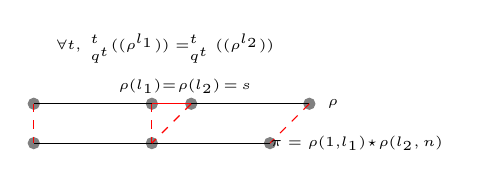
\begin{tikzpicture}
    				%				[->,>=stealth',shorten >=1pt,auto,node distance=0,main node/.style={circle,draw}]
    	\filldraw [gray] (0,0) circle (2pt)
    	(1.5,0) circle (2pt)
    	(2,0) circle (2pt)
    	(3.5,0) circle (2pt);
    	%
    	\filldraw [gray] (0,-0.5) circle (2pt)
    	(1.5,-0.5) circle (2pt)
    	(3,-0.5) circle (2pt);
    	%
    	\draw [red] (1.5,0) -- (2,0);
    	\draw [black]  (0,0) -- (1.5,0);
    	\draw [black] (2,0) -- (3.5,0);
    	\draw [black] (0,-0.5) -- (3,-0.5);
    	\draw [dashed, red] (0,0) -> (0,-0.5);
    	\draw [dashed, red] (1.5,0) -> (1.5,-0.5);
    	\draw [dashed, red] (2,0) -> (1.5,-0.5);
    	\draw [dashed, red] (3.5,0) -> (3,-0.5);
    	{\tiny
    		\node (a0) at (3.8,0) {$\rho$};	
    		\node (b0) at (4.1,-0.5) {$\pi=\rho(1,\! l_1)\!\star\! \rho(l_2,n)$};	
    		\node (a1) at (1.35,0.22) {$\rho(l_1)$};
    		\node (a11) at (1.72,0.22) {$=$};
    		\node (a2) at (2.1,0.22) {$\rho(l_2)$};
    		\node (a111) at (2.5,0.22) {$=$};
    		\node (a21) at (2.7,0.22) {$s$};
    		\node (a3) at (1.67,0.7) {$\forall t,\; \Du^t_{q^t}(\Lab(\rho^{l_1}))=\Du^t_{q^t}(\Lab(\rho^{l_2}))$};	
    	}
    \end{tikzpicture}}
    \caption{The contraction step of Proposition~\ref{proposition:wellFormdnessRegex}.}\label{fig:basicContrRegex}
\end{figure}


\section{Proof of Theorem~\ref{theorem:expSizeModelPropertyAAbarBBbarRegex}}\label{proof:theorem:expSizeModelPropertyAAbarBBbarRegex}

\begin{theorem*}[\ref{theorem:expSizeModelPropertyAAbarBBbarRegex}, Exponential small-model for $\AAbarBBbar$]
Let $\Ku=(\Prop,\States,\allowbreak \Edges,\Lab,\sinit)$ be a finite Kripke structure, $\sigma,\rho \in \Trk_\mathpzc{K}$, and $\varphi$ be an $\AAbarBBbar$ formula in \nnf{}, with $\RE$'s  $r_1,\ldots ,r_u$ over $\Prop$, such that $\Ku,\sigma\star\rho\models \varphi$. There exists $\pi\in \Trk_\mathpzc{K}$, induced by $\rho$, such that $\Ku,\sigma\star\pi\models \varphi$ and $|\pi|\leq |\States|\cdot (|\varphi|+1) \cdot 2^{2\sum_{\ell=1}^u |r_\ell|}$.
\end{theorem*}

\begin{proof} 
%W.l.o.g., we can restrict ourselves to set of proposition letters occurring in $\varphi$, thus assuming $|\Prop|\leq |\varphi|$. 
Let $Wt(\varphi,\sigma\star\rho)$ be the set of witness positions of $\sigma\star\rho$ for $\varphi$.
Let $\{i_1,\ldots,i_k\}$ be the ordering of $Wt(\varphi,\sigma\star\rho)$ such that
$i_1<\ldots <i_k$. Let $i_0=1$ and $i_{k+1}=|\sigma\star\rho|$. Hence, $1=i_0\leq  i_1<\ldots <i_k < i_{k+1}=|\sigma\star\rho|$.
%
If the length of $\rho$ is at most $|\States|\cdot (|\varphi|+1) \cdot 2^{2\sum_{\ell=1}^u |r_\ell|}$, the thesis trivially holds.
Let us assume that $|\rho|> |\States|\cdot (|\varphi|+1) \cdot 2^{2\sum_{\ell=1}^u |r_\ell|}$. We show that there exists a trace $\pi$ induced by $\rho$, with $|\pi| < |\rho |$, such that $\Ku,\sigma\star\pi\models \varphi$. 

W.l.o.g., we can assume that $i_0\leq i_1<\ldots <i_{j-1}$, for some $j\geq 1$, are $\sigma$-positions (while $i_{j}<\ldots <i_{k+1}$ are $(\sigma\star\rho)$-positions not in $\sigma$). We claim that either $(i)$~there exists $t\in [j,k]$ such that $i_{t+1}-i_t>|\States|\cdot 2^{2\sum_{\ell=1}^u |r_\ell|}$ or $(ii)$~$|(\sigma\star\rho)(|\sigma|,i_{j})|>|\States|\cdot 2^{2\sum_{\ell=1}^u |r_\ell|}$. By way of contradiction, suppose that neither $(i)$ nor $(ii)$ holds. We need to distinguish two cases. 
If $\sigma\star\rho=\rho$, then 
$|\rho| = (i_{k+1}-i_0)+1\leq (k+1) \cdot |\States|\cdot 2^{2\sum_{\ell=1}^u |r_\ell|} +1$ (a contradiction); 
otherwise ($|\rho| < |\sigma\star\rho|$), $|\rho| = (i_{k+1} - i_{j}) + |(\sigma\star\rho)(|\sigma|,i_{j})| \leq k \cdot |\States|\cdot 2^{2\sum_{\ell=1}^u |r_\ell|} + |\States|\cdot 2^{2\sum_{\ell=1}^u |r_\ell|} \leq (k+1) \cdot |\States|\cdot 2^{2\sum_{\ell=1}^u |r_\ell|}$. The contradiction follows since $(k+1) \cdot |\States|\cdot 2^{2\sum_{\ell=1}^u |r_\ell|}+1 \leq |\varphi| \cdot |\States|\cdot 2^{2\sum_{\ell=1}^u |r_\ell|}+1 \leq |\States|\cdot (|\varphi|+1)\cdot 2^{2\sum_{\ell=1}^u |r_\ell|}$.
%Otherwise, if neither $(i)$ nor $(ii)$ happens, then $|\rho|-1\leq i_{k+1}-i_0\leq (k+1)\cdot |W|\cdot (|\varphi|+1) < %|W|\cdot (|\varphi|+1)^2$, as $k\leq |\varphi|-1$. This contradicts the fact that $|\rho|> |W|\cdot (|\varphi|+1)^2$.
 
Let us define $(\alpha,\beta)=(i_t,i_{t+1})$ in case $(i)$, and $(\alpha,\beta)=(|\sigma|,i_{j})$ in case $(ii)$. Moreover let $\rho'=\rho(\alpha,\beta)$. In both the cases, we have  $|\rho'|> |\States|\cdot 2^{2\sum_{\ell=1}^u |r_\ell|}$.
%
By Proposition~\ref{proposition:wellFormdnessRegex}, there exists a trace $\pi'$ of $\Ku$, $(q^1,\ldots , q^u)$-well-formed with respect to $\rho'$, such that $|\pi'|\leq |\States|\cdot 2^{2\sum_{\ell=1}^u |r_\ell|} < |\rho'|$, 
where we choose $q^x=\Du^x(\Lab((\sigma\star\rho)^{\alpha-1}))$ for $x=1,\ldots , u$ (as a particular case we set $q^x$ as the initial state of $\Du^x$ if $\alpha=1$).
Let $\pi$ be the trace induced by $\rho$ obtained by replacing the subtrace $\rho'$ of $\rho$ with $\pi'$ (see Figure~\ref{fig:contr2Regex}). Since $|\pi|<|\rho|$, it remains to prove that  $\Ku,\sigma\star\pi\models \varphi$.

\begin{figure}[b]
\centering
    \resizebox{0.9\linewidth}{!}{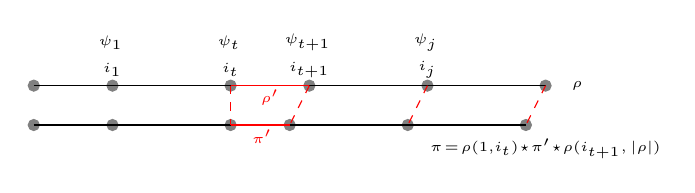
\begin{tikzpicture}
				%				[->,>=stealth',shorten >=1pt,auto,node distance=0,main node/.style={circle,draw}]
				\filldraw [gray] (0,0) circle (2pt)
				(1.0,0) circle (2pt)
				(2.5,0) circle (2pt)
				(3.5,0) circle (2pt) 
				(5.0,0) circle (2pt)
				(6.5,0) circle (2pt);
				%
				\filldraw [gray] (0,-0.5) circle (2pt)
				(1.0,-0.5) circle (2pt)
				(2.5,-0.5) circle (2pt)
				(3.25,-0.5) circle (2pt) 
				(4.75,-0.5) circle (2pt)
				(6.25,-0.5) circle (2pt);
				%
				\draw [red] (2.5,0) -- (3.5,0);
				\draw [black]  (0,0) -- (2.5,0);
				\draw [black] (3.5,0) -- (6.5,0);
				\draw [black] (0,-0.5) -- (2.5,-0.5);
				\draw [red] (2.5,-0.5) -- (3.25,-0.5);
				\draw [black] (3.25,-0.5) -- (6.25,-0.5);
				\draw [dashed, red] (2.5,0) -> (2.5,-0.5);
					\draw [dashed, red] (3.5,0) -> (3.25,-0.5);
				\draw [dashed, red] (5,0) -> (4.75,-0.5);
				\draw [dashed, red] (6.5,0) -> (6.25,-0.5);
				{\tiny
					\node (a0) at (6.9,0) {$\rho$};	
					\node (b0) at (6.5,-0.8) {$\pi\!=\!\rho(1,\! i_t)\!\star\! \pi'\! \star\! \rho(i_{t+1},|\rho|)$};	
					\node (a1) at (1,0.2) {$i_1$};
					\node (a2) at (2.5,0.2) {$i_t$};
					\node (a3) at (3.5,0.2) {$i_{t+1}$};
					\node (a4) at (5,0.2) {$i_{j}$};
					\node (a1) at (1,0.55) {$\hsB\! \psi_1$};
					\node (a2) at (2.5,0.55) {$\hsB\! \psi_{t}$};
					\node (a3) at (3.5,0.55) {$\hsB\! \psi_{t+1}$};
					\node (a4) at (5,0.55) {$\hsB\! \psi_{j}$};
					\node [red] (a4) at (2.9,-0.65) {$\pi'$};
					\node [red] (a4) at (3.0,-0.15) {$\rho'$};
				}
				
			\end{tikzpicture}}
    \caption{Representation of the contraction step of Theorem~\ref{theorem:expSizeModelPropertyAAbarBBbarRegex}---case $(i)$}\label{fig:contr2Regex}
\end{figure}

Let us denote $\sigma\star\pi$ by $\overline{\pi}$ and $\sigma\star\rho$ by $\overline{\rho}$. Moreover,
let $H:[1,|\overline{\pi}|] \rightarrow [1,|\overline{\rho}|]$ be the function mapping positions of $\overline{\pi}$ into positions of $\overline{\rho}$ in this way: positions ``outside'' $\pi'$ (i.e., outside the interval $[\alpha,\alpha+|\pi'|-1]$) are mapped into their original position in $\overline{\rho}$; positions ``inside'' $\pi'$ (i.e., in $[\alpha,\alpha+|\pi'|-1]$) are mapped to the corresponding position in 
$\rho'$ (exploiting well-formedness of $\pi'$ w.r.t.\ $\rho'$). Formally,  $H$ is defined as:
%
\begin{equation*}\label{equation:H}
H(m) = \begin{cases}  
	m& \text{if}\quad m<\alpha \\
\alpha+\ell_{m-\alpha+1}-1 & \mbox{if}\quad \alpha\leq m<\alpha+|\pi'| \\
m+(|\rho'| - |\pi'|) & \mbox{if}\quad m\geq \alpha+|\pi'|
\end{cases}
\end{equation*}
where  $\ell_m$ is the $\rho'$-position corresponding to the $\pi'$-position $m$.
%
It is easy to check that $H$ satisfies the following properties: 
\begin{enumerate}
    \item $H$ is strictly monotonic, i.e., for all $j,j'\in [1,|\overline{\pi}|]$, $j<j'\iff H(j)<H(j')$;
    \item for all $j\in [1,|\overline{\pi}|]$, $\overline{\pi}(j) = \overline{\rho}(H(j))$;
    \item $H(1)= 1$ and $H(|\overline{\pi}|)=|\overline{\rho}|$;
    \item $Wt(\varphi, \overline{\rho}) \subseteq \{H(j) \mid j \in [1,|\overline{\pi}|] \}$  i.e., all witness positions are preserved;
    \item for each $j\in [1,|\overline{\pi}|]$ and $x=1,\ldots , u$, $\Du^x(\Lab(\overline{\pi}^{j}))=\Du^x(\Lab(\overline{\rho}^{H(j)}))$.
\end{enumerate}
We only comment on Property~5.
The property holds for $j\in [1,\alpha-1]$, as $\overline{\pi}^j=\overline{\rho}^{H(j)}=\overline{\rho}^j$. 
For $j\in [\alpha,\alpha+|\pi'|-1]$, $\Du^x(\Lab(\overline{\pi}^j))=\Du^x(\Lab(\overline{\rho}^{H(j)}))$ follows from the well-formedness hypothesis.
Finally, being $\overline{\rho}(\beta,|\overline{\rho}|)=\overline{\pi}(\alpha+|\pi'|-1,|\overline{\pi}|)$ and $\Du^x(\Lab(\overline{\pi}^{\alpha+|\pi'|-1}))=\Du^x(\Lab(\overline{\rho}^\beta))$, the property holds also for $j\in [\alpha+|\pi'|,|\overline{\pi}|]$.

The fact that
$\Ku,\overline{\pi}\models \varphi$ is an immediate consequence of the following claim, considering that  $H(|\overline{\pi}|)=|\overline{\rho}|$, $\Ku,\overline{\rho}\models \varphi$,  $\overline{\rho}^{|\overline{\rho}|}=\overline{\rho}$, and $\overline{\pi}^{|\overline{\pi}|}=\overline{\pi}$.

\begin{claim}\label{claim:Hj} For all $j\in [1,|\overline{\pi}|]$, all subformulas $\psi$ of $\varphi$, and all $\xi\in\Trk_\Ku$, 
it holds that
$
\Ku,\overline{\rho}^{H(j)}\star \xi\models \psi \Longrightarrow \Ku,\overline{\pi}^{j}\star \xi\models \psi.
$
\end{claim}
\begin{proof}
Assume that $\Ku,\overline{\rho}^{H(j)}\star \xi\models \psi $. Note that $\overline{\rho}^{H(j)}\star \xi$ is defined if and only if $\overline{\pi}^{j}\star \xi$ is defined. We prove by induction on the structure of $\psi$  that
$\Ku,\overline{\pi}^{j}\star \xi\models \psi$. Since $\varphi$ is in \nnf, only the following cases can occur.

\begin{itemize}
  \item $\psi= r_t$ or $\psi=\neg r_t$ where $r_t$ is some $\RE$ over $\Prop$. By Property~5 of $H$, 
   $\Du^t(\Lab(\overline{\pi}^j))=\Du^t(\Lab(\overline{\rho}^{H(j)}))$, thus $\Du^t(\Lab(\overline{\pi}^j\star \xi))=\Du^t(\Lab(\overline{\rho}^{H(j)}\star \xi))$. It follows that
    $\Ku, \overline{\pi}^{j}\star \xi \models r_t$ if and only if $\Ku,\overline{\rho}^{H(j)}\star \xi \models r_t$, and the thesis holds.
%
    \item $\psi= \theta_1\wedge\theta_2$ or $\psi= \theta_1\vee\theta_2$ for some $\AAbarBBbar$ formulas $\theta_1$ and $\theta_2$. 
    The result holds by the inductive hypothesis.
%
   \item $\psi = \hsBu\theta$. We need to show that for each proper prefix $\eta$ of $\overline{\pi}^{j}\star \xi$, we have $\Ku,\eta\models\theta$. We distinguish two cases:
     \begin{itemize}
       \item $\eta$ is \emph{not} a proper prefix of $\overline{\pi}^{j}$. Hence, $\eta$ has the form $ \overline{\pi}^{j}\star \xi^h$ for some $h\in [1,|\xi|-1]$. Since $\Ku,\overline{\rho}^{H(j)}\star \xi\models \hsBu\theta $, then
       $\Ku,\overline{\rho}^{H(j)}\star \xi^h\models \theta $.  By the inductive hypothesis, we have $\Ku,\overline{\pi}^j\star \xi^h\models \theta $.
       \item $\eta$ is a proper prefix of $\overline{\pi}^{j}$. Hence, $\eta = \overline{\pi}^{h}$ for some $h\in [1,j-1]$.   By Property~1 of $H$, $H(h)<H(j)$, and since $\Ku,\overline{\rho}^{H(j)}\star \xi\models \hsBu\theta $, we have that $\Ku,\overline{\rho}^{H(h)}\models \theta $. By the inductive hypothesis, $\Ku,\overline{\pi}^h\models \theta $.
     \end{itemize}
    Therefore, $\Ku,\overline{\pi}^j\star \xi\models \hsBu\theta $ holds.
%
    \item $\psi = \hsB\theta$. We have to show that there exists a proper prefix of $\overline{\pi}^{j}\star \xi$ satisfying $\theta$.
Since $\Ku,\overline{\rho}^{H(j)}\star \xi\models \psi $, there exists a proper prefix $\eta'$ of  $\overline{\rho}^{H(j)}\star \xi$
 such that  $\Ku,\eta'\models \theta $. We distinguish two cases:
 \begin{itemize}
   \item $\eta'$ is \emph{not} a proper prefix of $\overline{\rho}^{H(j)}$. Hence, $\eta'$ is of the form $\overline{\rho}^{H(j)}\star \xi^h$ for some $h\in [1,|\xi|-1]$. By the inductive hypothesis, $\Ku,\overline{\pi}^j\star \xi^h\models \theta $, hence $\Ku,\overline{\pi}^j\star \xi\models \hsB\theta $.
   \item $\eta'$ is a proper prefix of $\overline{\rho}^{H(j)}$. Hence, $\eta' = \overline{\rho}^{i}$ for some $i\in [1,H(j)-1]$, and $\Ku,\overline{\rho}^{i}\models \theta $.
   Let $i'$ be the smallest position of $\overline{\rho}$ such that $\Ku,\overline{\rho}^{i'}\models\theta$. Hence $i'\leq i$ and $i'\in Wt(\varphi,\overline{\rho})$. By Property~4 of $H$, $i'=H(h)$ for some $\overline{\pi}$-position $h$. Since $H(h)<H(j)$, it holds that $h<j$ (Property~1). By the inductive hypothesis, $\Ku,\overline{\pi}^h\models \theta $, and thus $\Ku,\overline{\pi}^j\star \xi\models \hsB\theta $.
 \end{itemize}
 Therefore, in both cases, $\Ku,\overline{\pi}^j\star \xi\models \hsB\theta$.
% 
    \item $\psi=\hsBtu\theta$ or $\psi=\hsBt\theta$. The thesis directly follows from the inductive hypothesis.
%
    \item $\psi = \hsAu\theta$, $\psi=\hsA\theta$, $\psi = \hsAtu\theta$ or $\psi=\hsAt\theta$. Since $\overline{\pi}^j\star \xi$ and $\overline{\rho}^{H(j)}\star \xi$ start at the same state and lead to the same state (by Property~2 and 3 of $H$), the result trivially follows. This concludes the proof of the claim.\qedhere
\end{itemize}
\end{proof}

We have shown that $\Ku,\overline{\pi}\models \varphi$, with $|\pi| < |\rho |$. If $|\pi|\leq |\States|\cdot (|\varphi|+1)\cdot 2^{2\sum_{\ell=1}^u |r_\ell|}$, the thesis holds. Otherwise, we can iterate the above contraction a finite number of times until the bound is reached.
\end{proof}


\section{Proof of Theorem~\ref{corrComplCheckBBbar}}\label{proof:corrComplCheckBBbar}

\begin{theorem*}[\ref{corrComplCheckBBbar}]
Let $\Phi$ be a $\B\Bbar$ formula, $\psi$ be a subformula of $\Phi$, and $\rho\in\Trk_{\Ku}$ be a trace with $s=\lst(\rho)$. Let $G$ be the subset of formulas in $\subfB(\psi)$ that hold on some proper prefix of $\rho$.
Let $\Du(\Phi)$ be the current configuration of the $\DFA$s associated with the regular expressions in $\Phi$ after reading $\mu(\rho(1,|\rho|-1))$.
%(i.e., $\mu(\rho)$ but the last symbol).
%
Then $\texttt{Check}(\Ku,\psi,s,G,\Du(\Phi))=\top \!\iff\! \Ku,\rho\models \psi$.
\end{theorem*}

\begin{proof}
The proof is by induction on the structure of $\psi$. The thesis trivially follows for the cases $\psi=r$ (regular expression), $\psi=\neg\psi'$, $\psi=\psi_1\wedge\psi_2$, and $\psi=\hsB\psi'$.

Let us now assume $\psi=\hsBt\psi'$. 
\texttt{Check}$(\Ku,\psi,s,G,\Du(\Phi))=\top$ if and only if, for some $b''\in\{1,\ldots , |\States|\cdot (2|\psi'|+1)\cdot 2^{2\sum_{\ell=1}^u |r_\ell|}-1 \}$ and some $(G'',\Du(\Phi)'',s'')\in\conf(\Ku,\psi)$ ($=\conf(\Ku,\psi')$), we have \texttt{Reach}$(\Ku,\psi',(G,\Du(\Phi),s),(G'',\Du(\Phi)'', s''),\allowbreak b'')=\top$ and \texttt{Check}$(\Ku,\psi',s'',G'', \Du(\Phi)'')=\top$.
We preliminary prove the following claim.
    \begin{claim}
        Let $b\in\mathbb{N}$, $b>0$.
        Let $\tilde{\rho}\in\Trk_{\Ku}$ be a trace with $\tilde{s}=\lst(\tilde{\rho})$. Let $\tilde{G}$ be the subset of formulas in $\subfB(\psi')$ that hold on some proper prefix of $\tilde{\rho}$.
        Let $\tilde{\Du}(\Phi)$ be the current configuration of states of the $\DFA$s associated with the regular expressions in $\Phi$, reached from the initial states after reading $\Lab(\tilde{\rho}(1,|\tilde{\rho}|-1))$.
        
        For $(\tilde{G},\tilde{\Du}(\Phi),\tilde{s})$, $(G',\Du(\Phi)',s')\in\conf(\Ku,\psi')$, we have 
        \texttt{Reach}$(\Ku,\psi',\allowbreak (\tilde{G},\tilde{\Du}(\Phi),\tilde{s}),\allowbreak (G',\Du(\Phi)',s'),b)=\top$ if and only if there exists $\rho'\in\Trk_{\Ku}$ such that $\tilde{\rho}\cdot\rho'\in\Trk_\Ku$, $|\rho'|=b$, $\lst(\rho')=s'$, $G'$ is the subset of formulas in $\subfB(\psi')$ that hold on some proper prefix of $\tilde{\rho}\cdot\rho'$, and $\Du(\Phi)'$ is the current configuration of the $\DFA$s associated with the regular expressions of $\Phi$, after reading $\Lab(\tilde{\rho}\cdot\rho'(1,|\tilde{\rho}\cdot\rho'|-1))$.
    \end{claim}
    \begin{proof}
    The proof is by induction on $b\geq 1$.
    
    If $b\!=\!1$ we have \texttt{Reach}$(\Ku,\psi',(\tilde{G},\tilde{\Du}(\Phi),\tilde{s}),(G',\Du(\Phi)',s'),b)\!=\!\top$ if and only if  \texttt{Compatible}($\Ku,\psi',\allowbreak (\tilde{G},\tilde{\Du}(\Phi),\tilde{s}),(G',\Du(\Phi)',s'))\!=\!\top$; this happens if and only if: \begin{enumerate}
        \item[1.] $(\tilde{s},s')\in \Edges$, i.e., $(\tilde{s},s')$ is an edge of $\Ku$;
        \item[2.] \texttt{advance}$(\tilde{\Du}(\Phi),\Lab(\tilde{s}))=\Du(\Phi)'$;
        \item[3.] $\tilde{G}\subseteq G'$;
        \item[4.] for each $\varphi\in(G'\setminus \tilde{G})$, \texttt{Check}$(\Ku,\varphi,\tilde{s},\tilde{G}\cap \subfB(\varphi),\tilde{\Du}(\Phi))=\top$;
        \item[5.] for each $\varphi\in(\subfB(\psi')\setminus G')$, \texttt{Check}$(\Ku,\varphi,\tilde{s},\tilde{G}\cap \subfB(\varphi),\tilde{\Du}(\Phi))=\bot$.
    \end{enumerate}
    Let $\rho'=s'$. ($\Rightarrow$)
    By the inductive hypothesis (of the external theorem over $\tilde{\rho}$), by (4.) it follows that $\Ku,\tilde{\rho}\models\varphi$ for each $\varphi\in(G'\setminus \tilde{G})$. By (5.) it follows that $\Ku,\tilde{\rho}\not\models\varphi$ for each  $\varphi\in(\subfB(\psi')\setminus G')$ and the claim follows.

     ($\Leftarrow$) Conversely (1.), (2.), and (3.) easily follow. Moreover, it must hold that $\Ku,\tilde{\rho}\models\varphi$ for each $\varphi\in (G'\setminus \tilde{G})$, and $\Ku,\tilde{\rho}\not\models\varphi$ for each  $\varphi\in (\subfB(\psi')\setminus G')$ and, therefore, (4.) and (5.) follow by the inductive hypothesis (of the external theorem).
    
    If $b\geq 2$, \texttt{Reach}$(\Ku,\psi',(\tilde{G},\tilde{\Du}(\Phi),\tilde{s}),(G',\Du(\Phi)',s'),b)=\top$ if and only if, for some $(G_3,\Du(\Phi)_3,s_3)\in\conf(\Ku,\psi')$,  \texttt{Reach}($\Ku,\psi',(\tilde{G},\tilde{\Du}(\Phi),\tilde{s}),(G_3,\Du(\Phi)_3,s_3), \linebreak \lfloor b/2\rfloor)=\top$ and  \texttt{Reach}($\Ku,\psi',(G_3,\Du(\Phi)_3,s_3),(G',\Du(\Phi)',s'),b-\lfloor b/2\rfloor)=\top$.
    
    ($\Rightarrow$) By the inductive hypothesis (over $b$), there exists $\rho_3\in\Trk_{\Ku}$ such that $\tilde{\rho}\cdot\rho_3\in\Trk_\Ku$, $|\rho_3|=\lfloor b/2\rfloor$, $\lst(\rho_3)=s_3$, $G_3$ is the subset of subformulas in $\subfB(\psi')$ that hold on some proper prefix of $\tilde{\rho}\cdot\rho_3$, and $\Du(\Phi)_3$ is the current configuration of the $\DFA$s associated with the regular expressions in $\Phi$, after reading $\Lab(\tilde{\rho}\cdot\rho_3(1,|\tilde{\rho}\cdot\rho_3|-1))$.
    
    By the inductive hypothesis (over $b$, applied to the trace $\tilde{\rho}\cdot\rho_3$), there exists $\rho'\in\Trk_{\Ku}$ such that $\tilde{\rho}\cdot\rho_3\cdot \rho'\in\Trk_\Ku$, $|\rho'|=b-\lfloor b/2\rfloor$, $\lst(\rho')=s'$, $G'$ is the subset of subformulas in $\subfB(\psi')$ that hold on some proper prefix of $\tilde{\rho}\cdot\rho_3\cdot \rho'$, and $\Du(\Phi)'$ is the current configuration of the $\DFA$s associated with the regular expressions in $\Phi$, after reading $\Lab(\tilde{\rho}\cdot\rho_3\cdot \rho'(1,|\tilde{\rho}\cdot\rho_3\cdot \rho'|-1))$.
    %
    The claim follows, as $\rho_3\cdot\rho'\in\Trk_\Ku$ and $|\rho_3\cdot\rho'|=b$.
    
    ($\Leftarrow$)
    Conversely, there exists $\rho'\in\Trk_{\Ku}$ such that $\tilde{\rho}\cdot\rho'\in\Trk_\Ku$, $|\rho'|=b\geq 2$, $\lst(\rho')=s'$, $G'$ is the subset of subformulas in $\subfB(\psi')$ that hold on some proper prefix of $\tilde{\rho}\cdot\rho'$, and $\Du(\Phi)'$ is the current configuration of the $\DFA$s associated with the regular expressions in $\Phi$, after reading $\Lab(\tilde{\rho}\cdot\rho'(1,|\tilde{\rho}\cdot\rho'|-1))$.
    Let us split $\rho'=\rho_3\cdot\rho_4$, where $|\rho_3|=\lfloor b/2\rfloor$ and $|\rho_4|=b-\lfloor b/2\rfloor$.
    Let $(G_3,\Du(\Phi)_3,s_3)\in\conf(\Ku,\psi')$ be such that $\Du(\Phi)_3$ is the current configuration of the $\DFA$s associated with the regular expressions in $\Phi$, after reading $\Lab(\tilde{\rho}\cdot\rho_3(1,|\tilde{\rho}\cdot\rho_3|-1))$, $s_3=\lst(\rho_3)$, $G_3$ is the subset of subformulas in $\subfB(\psi')$ that hold on some proper prefix of $\tilde{\rho}\cdot\rho_3$. By the inductive hypothesis (on $b$ over $\tilde{\rho}\cdot\rho_3$), 
    \texttt{Reach}($\Ku,\psi',(G_3,\Du(\Phi)_3,s_3),(G',\Du(\Phi)',s'),b-\lfloor b/2\rfloor)=\top$.
    Moreover, by the inductive hypothesis (on $b$ over $\tilde{\rho}$), we have
    \texttt{Reach}($\Ku,\psi',(\tilde{G},\tilde{\Du}(\Phi),\tilde{s}),(G_3,\Du(\Phi)_3,s_3),\allowbreak \lfloor b/2\rfloor)=\top$.
    
    Hence, both the recursive calls at line 6 return $\top$, when at line 5 $(G_3,\Du(\Phi)_3,s_3)$ is considered by the loop. Thus, \texttt{Reach}$(\Ku,\psi',(\tilde{G},\tilde{\Du}(\Phi),\tilde{s}),(G',\Du(\Phi)',s'),b)$ returns $\top$ concluding the proof of the claim.
    \end{proof}
    
    ($\Rightarrow$)
    Let us now assume that in the execution of \texttt{Check}, at lines 15--19, for some $b''\in\{1,\ldots , |\States|\cdot (2|\psi'|+1)\cdot 2^{2\sum_{\ell=1}^u |r_\ell|}-1 \}$ and some $(G'',\Du(\Phi)'',s'')\in\conf(\Ku,\psi)$ ($=\conf(\Ku,\psi')$), we have \texttt{Reach}$(\Ku,\psi',(G,\Du(\Phi),s),(G'',\Du(\Phi)'',s''),\allowbreak b'')=\top$ and \texttt{Check}$(\Ku,\psi',s'',\allowbreak G'',\Du(\Phi)'')=\top$. By the claim above, there exists $\rho''\in\Trk_{\Ku}$ such that $\rho\cdot\rho''\in\Trk_\Ku$, $\lst(\rho'')=s''$, $G''$ is the subset of subformulas in $\subfB(\psi')$ that hold on some proper prefix of $\rho\cdot\rho''$, and $\Du(\Phi)''$ is the current configuration of the $\DFA$s associated with the regular expressions of $\Phi$, after reading $\Lab(\rho\cdot\rho''(1,|\rho\cdot\rho''|-1))$.
%    
    By the inductive hypothesis, since \texttt{Check}$(\Ku,\psi',s'',G'',\Du(\Phi)'')=\top$, we have $\Ku,\rho\cdot\rho''\models \psi'$ implying that $\Ku,\rho\models \hsBt\psi'$.
    
    ($\Leftarrow$)
    Conversely, if $\Ku,\rho\models \hsBt\psi'$, we have $\Ku,\rho\cdot\rho''\models \psi'$ for some $\rho''\in\Trk_\Ku$, with $\rho\cdot\rho''\in\Trk_\Ku$. By the exponential small-model property (Theorem~\ref{theorem:expSizeModelPropertyAAbarBBbarRegex}), there exists $\rho'\in\Trk_\Ku$ such that $\lst(\rho'')=\lst(\rho')$, $|\rho'|\leq |\States|\cdot (2|\psi'|+1)\cdot 2^{2\sum_{\ell=1}^u |r_\ell|}-1$ (recall that the factor 2 in front of $|\psi'|$ is due to the fact that 
    %the exponential small-model property requires 
    a formula in \nnf{} is required), $\rho\cdot\rho'\in\Trk_\Ku$ and $\Ku,\rho\cdot\rho'\models \psi'$. Let $G'$ be the subset of subformulas in $\subfB(\psi')=\subfB(\psi)$ that hold on some proper prefix of $\rho\cdot\rho'$, and $\Du(\Phi)'$ be the current configuration of the $\DFA$s associated with the regular expressions in $\Phi$, after reading $\Lab(\rho\cdot\rho'(1,|\rho\cdot\rho'|-1))$. By the inductive hypothesis (over $\rho\cdot\rho'$), \texttt{Check}$(\Ku,\psi',\lst(\rho'),G',\Du(\Phi)')=\top$.
    By the claim above, \texttt{Reach}$(\Ku,\psi',(G,\Du(\Phi),s), (G',\Du(\Phi)',\lst(\rho')),\allowbreak |\rho'|)=\top$, hence \texttt{Check}$(\Ku,\psi,s,G,\Du(\Phi))=\top$.
    %
    This concludes the proof of the theorem.
\end{proof}


\section{Proof of Theorem~\ref{corrCheckAux}}\label{proof:corrCheckAux}

\begin{theorem*}[\ref{corrCheckAux}]
    Let $\Ku=\KuDef$ be a finite Kripke structure, and $\Phi$ be a $\B\Bbar$ formula. Then, \texttt{CheckAux}$(\Ku,\Phi)=\top\iff\Ku\models\Phi$.
\end{theorem*}

\begin{proof}
    If $\Ku\models\Phi$, then for all $\rho\in\Trk_\Ku$ with $\fst(\rho)=\sinit$, we have $\Ku,\rho\models\Phi$. Hence, we have $\Ku,\sinit\models\Phi$, and $\Ku,\sinit\cdot\rho'\models\Phi$ for all $\sinit\cdot\rho'\in\Trk_\Ku$, implying that $\Ku,\sinit\models\hsBtu\Phi$ and $\Ku,\sinit\not\models\hsBt\neg\Phi$. By Theorem~\ref{corrComplCheckBBbar}, \texttt{Check}$(\Ku,\neg\Phi,\sinit,\emptyset,\Du(\Phi)_0)=\bot$ and  \texttt{Check}$(\Ku,\hsBt\neg\Phi,\sinit,\emptyset,\Du(\Phi)_0)=\bot$ implying that \texttt{CheckAux}($\Ku,\Phi)=\top$.
   
    Conversely, if \texttt{CheckAux}($\Ku,\Phi) = \top$, it must be \texttt{Check}$(\Ku,\neg\Phi,\sinit,\emptyset,\Du(\Phi)_0)=\bot$ and  \texttt{Check}$(\Ku,\hsBt\neg\Phi,\sinit,\emptyset,\Du(\Phi)_0)=\bot$. By Theorem~\ref{corrComplCheckBBbar} applied to the trace $\rho=\sinit$, we have $\Ku,\sinit\not\models\neg\Phi$ and $\Ku,\sinit\not\models\hsBt\neg\Phi$, and thus $\Ku\models\Phi$.
\end{proof}


\section{Proof of Theorem \ref{th:hard}}\label{sec:th:hard}

\begin{theorem*}[\ref{th:hard}]
The MC problem for $\HSprop$ formulas extended with regular expressions over finite Kripke structures is $\Psp$-hard (under polynomial-time reductions).
\end{theorem*}

\begin{proof}
    Given a regular expression $r$ with $\lang(r)\subseteq \Sigma^*$,
let us define the finite Kripke structure $\Ku=(\Sigma, \{\sinit\}\cup \Sigma, \Edges, \Lab, \sinit)$, where $\sinit\not\in \Sigma$, $\Lab(\sinit)=\emptyset$, for $c\in\Sigma$,  $\Lab(c)=\{c\}$, and $\Edges=\{(\sinit,c)\mid c\in\Sigma\}\cup \{(c,c')\mid c,c'\in \Sigma\}$.

It is easy to see that \[\lang(r)=\Sigma^*\iff \Ku\models \top\cdot \overline{r},\]
where 
$\overline{r}$ is a $\RE$ over $\Sigma$, \emph{syntactically} equal to $r$
(i.e., having exactly the same structure as $r$).
%
Note that even though if $r$ and $\overline{r}$ are syntactically equal,  $r$ is a regular expression defining a finitary language over $\Sigma$, whereas $\overline{r}$ defines a finitary language \emph{over $2^\Sigma$} (see Section~\ref{sect:backgrRegex}). The different notations  $r$ and $\overline{r}$ are kept to avoid confusion between the two different semantics.


    We show by induction on the structure of $r$ that, for all $w\in\Sigma^*$, $w \in\lang(r)\iff\Ku,w \models \overline{r}$.
The thesis follows as $\Ku,w \models \overline{r}$ if and only if $\Ku,\sinit\cdot w \models \top\cdot \overline{r}$.
%
\begin{itemize}
    \item $r=\varepsilon$. We have $w \in\lang(\varepsilon)$ if and only if $w=\varepsilon$, if and only if $\Lab(w)\in\lang(\overline{\varepsilon})=\{\varepsilon\}$, if and only if $\Ku,w\models \overline{\varepsilon}$.
%  
    \item $r=c\in\Sigma$. We have $w \in\lang(c)$ if and only if $w=c$, thus $\Lab(w)=\{c\}\in\lang(\overline{c})$, and $\Ku,w\models \overline{c}$. Conversely, if $\Ku,w\models \overline{c}$, we have $\Lab(w)\in\lang(\overline{c})=\{A\in 2^\Sigma\mid c\in A\}$. In particular $|w|=1$. Moreover, by definition of $\Lab$, $\Lab(w)$ is a singleton, hence $\Lab(w)=\{c\}$. By definition of $\Ku$, we get $w=c$, thus $w \in\lang(c)$.
%
    \item $r=r_1\cdot r_2$. We have $w \in\lang(r_1\cdot r_2)$ if and only if $w=w_1\cdot w_2$, with $w_1 \in\lang(r_1)$ and $w_2 \in\lang(r_2)$. By applying the inductive hypothesis, $\Ku,w_1 \models \overline{r_1}$ and $\Ku,w_2 \models \overline{r_2}$, thus $\Lab(w_1)\in\lang(\overline{r_1})$ and $\Lab(w_2)\in\lang(\overline{r_2})$. It follows that $\Lab(w)=\Lab(w_1)\cdot\Lab(w_2)\in\lang(\overline{r_1})\cdot\lang(\overline{r_2})=\lang(\overline{r_1\cdot r_2})$, namely, $\Ku,w\models \overline{r_1\cdot r_2}$.
    Conversely, $\Lab(w)\in\lang(\overline{r_1\cdot r_2})=\lang(\overline{r_1})\cdot\lang(\overline{r_2})$. Hence $\Lab(w_1)\in\lang(\overline{r_1})$ and $\Lab(w_2)\in\lang(\overline{r_2})$, for some $w_1\cdot w_2=w$. By the inductive hypothesis, $w_1\in\lang(r_1)$ and $w_2\in\lang(r_2)$, hence $w \in\lang(r_1\cdot r_2)$.
%  
    \item $r=r_1\cup r_2$. We have $w \in\lang(r_1\cup r_2)$ if and only if $w \in\lang(r_i)$ for some $i=1,2$. By the inductive hypothesis this is true if and only if $\Ku,w \models \overline{r_i}$, if and only if $\Lab(w) \in\lang(\overline{r_i})$, if and only if $\Lab(w) \in\lang(\overline{r_1\cup r_2})$, if and only if $\Ku,w \models \overline{r_1\cup r_2}$.
%
    \item $r=r_1^*$. 
 The thesis trivially holds if $w=\varepsilon$. 
    Let us now assume that $w\neq\varepsilon$. We have  $w \in\lang(r_1^*)$ if and only if, for some $t\geq 1$, $w=w_1\cdots w_t$ and $w_\ell\in\lang(r_1)$ for all $1\leq \ell\leq t$. By the inductive hypothesis, $\Ku,w_\ell \models \overline{r_1}$, thus $\Lab(w_\ell)\in\lang(\overline{r_1})$, and $\Lab(w)\in\lang(\overline{r_1^*})$. We conclude that $\Ku,w \models \overline{r_1^*}$. Conversely, $\Lab(w)\in\lang(\overline{r_1^*})=(\lang(\overline{r_1}))^*$, hence it must be the case that, for some $t\geq 1$, $w=w_1\cdots w_t$ and $\Lab(w_\ell)\in\lang(\overline{r_1})$  for all $1\leq \ell\leq t$. By the inductive hypothesis, $w_\ell\in\lang(r_1)$, hence $w\in\lang(r_1^*)$.
\end{itemize}
Finally, by observing that $\Ku$ can be built in polynomial time, the thesis follows.
\end{proof}